%%%%%%%%%%%%%%%%%%%%%%%%%%%%%%%%%%%%%%%%%%%%%%%%%%%%%%%%%%%%%%%%%%%%%%
% Overleaf (WriteLaTeX) Example: Molecular Chemistry Presentation
%
% Source: http://www.overleaf.com
%
% In these slides we show how Overleaf can be used with standard 
% chemistry packages to easily create professional presentations.
% 
% Feel free to distribute this example, but please keep the referral
% to overleaf.com
% 
%%%%%%%%%%%%%%%%%%%%%%%%%%%%%%%%%%%%%%%%%%%%%%%%%%%%%%%%%%%%%%%%%%%%%%

\documentclass{beamer}

\mode<presentation>
{
  \usetheme{Madrid}       % or try default, Darmstadt, Warsaw, ...
  \usecolortheme{default} % or try albatross, beaver, crane, ...
  \usefonttheme{default}    % or try default, structurebold, ...
  \setbeamertemplate{navigation symbols}{}
  \setbeamertemplate{caption}[numbered]
} 

\usepackage[english]{babel}
\usepackage[utf8x]{inputenc}
\usepackage{chemfig}
\usepackage[version=3]{mhchem}

\usepackage{hyperref}
  \hypersetup{colorlinks=true}
  \hypersetup{urlcolor=blue}
  \hypersetup{linkcolor = .}
\usepackage{xcolor}
\usepackage{siunitx}
  \sisetup{separate-uncertainty = true}
\usepackage{physics}
\usepackage[font=small,labelfont=bf]{caption}
\usepackage{subcaption}
\usepackage[en-GB]{datetime2}
\usepackage{overpic}
\usepackage{feynmp}
\DeclareGraphicsRule{*}{mps}{*}{}

\usepackage{scalerel}
\newcommand{\mylbrace}[2]{\vspace{#2pt}\hspace{6pt}\scaleleftright[\dimexpr5pt+#1\dimexpr0.06pt]{\lbrace}{\rule[\dimexpr2pt-#1\dimexpr0.5pt]{-4pt}{#1pt}}{.}}
\newcommand{\myrbrace}[2]{\vspace{#2pt}\scaleleftright[\dimexpr5pt+#1\dimexpr0.06pt]{.}{\rule[\dimexpr2pt-#1\dimexpr0.5pt]{-4pt}{#1pt}}{\rbrace}\hspace{6pt}}

% Here's where the presentation starts, with the info for the title slide
\title[$B^\pm\to(K^+K^-\pi^+\pi^-)_DK^\pm$]{\texorpdfstring{$\gamma$}{gamma} analysis update in \texorpdfstring{$B^\pm\to(K^+K^-\pi^+\pi^-)_DK^\pm$}{B to K+K-pi+pi-} decays}
\author{Martin Tat}
\institute{Oxford LHCb}
\date{28th June 2021}

\titlegraphic{
\includegraphics[height = 3cm, width = 4cm]{lhcb.jpg}\hspace{2cm}~%
              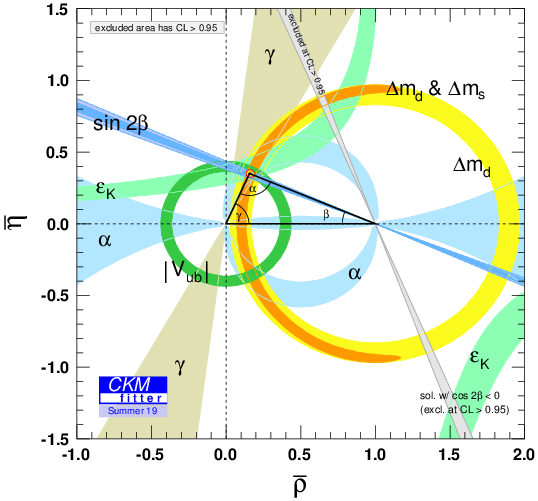
\includegraphics[height = 3cm, width = 4cm]{ckmfitter.png}}

\begin{document}

\begin{frame}
  \titlepage
\end{frame}

\begin{frame}{Summary of last time}
  \begin{itemize}
    \setlength\itemsep{1.5em}
    \item{$\gamma$ from $B^\pm\to DK^\pm$, $D\to K^+K^-\pi^+\pi^-$, \href{https://arxiv.org/abs/hep-ph/0611272}{arXiv:hep-ph/0611272}}
    \item{Model independent measurement with BESIII strong phase input}
    \item{Expected precision from signal-only study: $\Delta\gamma = \SI{12}{\degree}$}
    \item{$B$ candidate selection with BDT}
    \item{Currently only Run $2$}
    \item{Inital mass fits}
  \end{itemize}
\end{frame}

\begin{frame}{Summary of analysis procedure}
  \begin{enumerate}
    \setlength\itemsep{1.5em}
      \item{Perform global fit to fix yields and shapes}
      \item{Separate $B^\pm$ candidates by charge and into bins}
      \item{Extract $x_\pm$ and $y_\pm$ with a simultaneous fit}
      \item{Interpret $x_\pm$ and $y_\pm$ in terms of $\gamma$}
  \end{enumerate}
  \begin{block}{CP observables}
    $x_\pm = r_B^{DK}\cos(\delta_B^{DK}\pm\gamma), \quad y_\pm = r_B^{DK}\sin(\delta_B^{DK}\pm\gamma)$ \\
    $x_\xi^{D\pi} = \Re(\xi^{D\pi}), \quad y_\xi^{D\pi} = \Im(\xi^{D\pi}), \quad \xi^{D\pi} = \frac{r_B^{D\pi}}{r_B^{DK}}e^{i(\delta_B^{D\pi} - \delta_B^{DK})}$
  \end{block}
\end{frame}

% These three lines create an automatically generated table of contents.
\begin{frame}{Outline}
  \tableofcontents
\end{frame}

\section{Backgrounds}
\subsection{Mis-ID from \texorpdfstring{$D\to K\pi\pi\pi$}{D to Kpipipi}}
\begin{frame}{Mis-ID from $D\to K\pi\pi\pi$}
  \begin{itemize}
    \item{Mis-ID of $D$ daughter $\pi\to K$}
    \item{Peaks a much higher $D$ mass}
    \item{Much higher branching ratio}
    \item{Similar background from $D\to\pi\pi\pi\pi$ is negligible}
  \end{itemize}
  \begin{figure}
    \centering
    \vspace{-0.2cm}
    \begin{subfigure}{0.5\textwidth}
      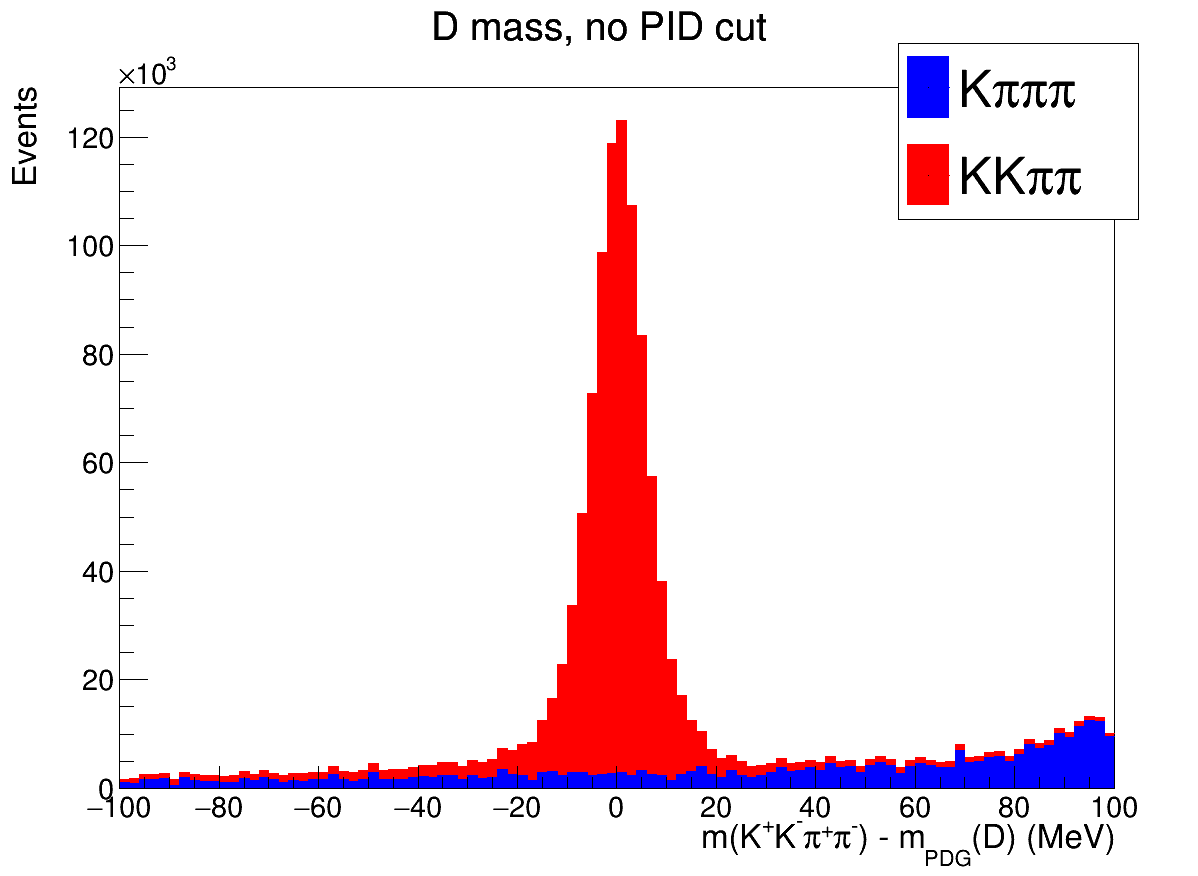
\includegraphics[width = 1.0\textwidth]{B2DK_Dmass_Background.png}
      \caption{$D$ invariant mass for $KK\pi\pi$ and $K\pi\pi\pi$}
    \end{subfigure}%
    \begin{subfigure}{0.5\textwidth}
      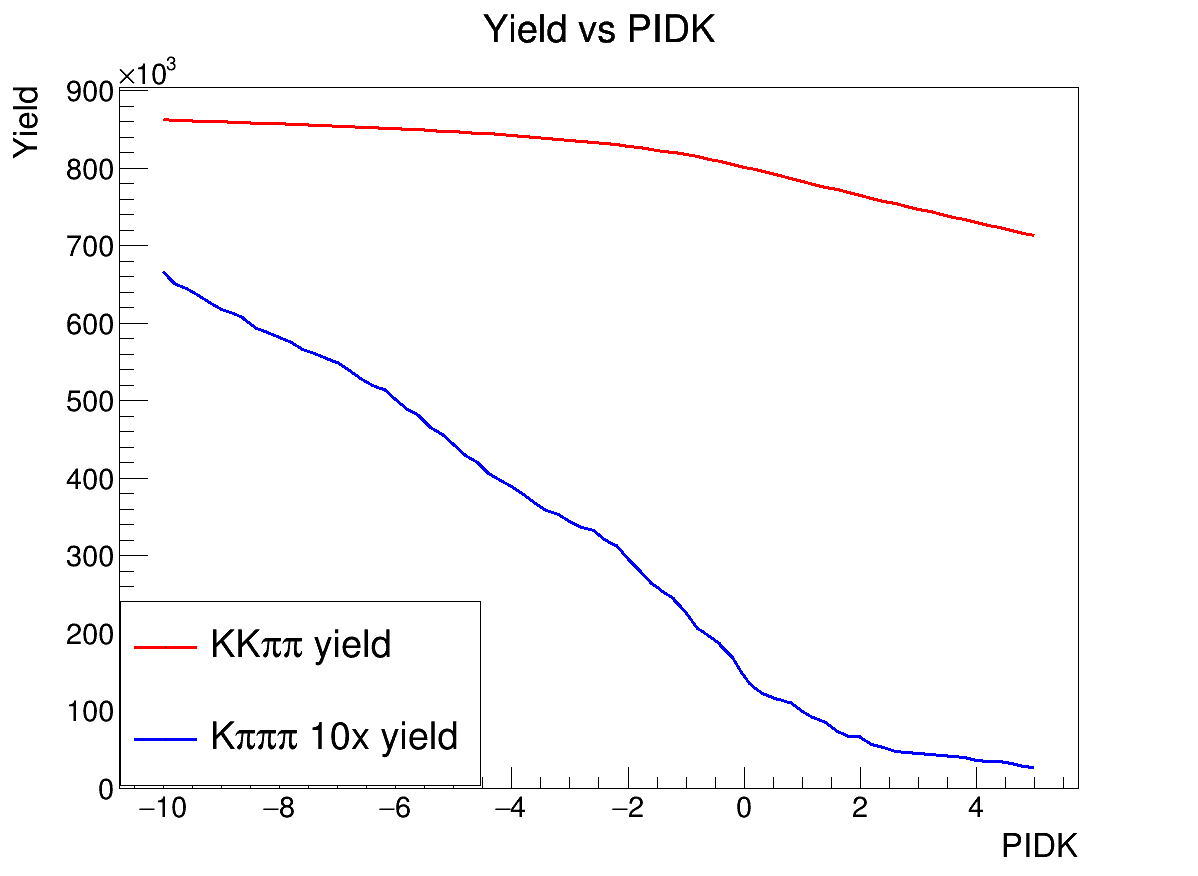
\includegraphics[width = 1.0\textwidth]{YieldVSPIDK.png}
      \caption{Yield of $KK\pi\pi$ and $K\pi\pi\pi$ vs $\text{PIDK}$}
    \end{subfigure}
  \end{figure}
\end{frame}

\subsection{Charmless backgrounds}
\begin{frame}{Charmless backgrounds}
  \begin{itemize}
    \setlength\itemsep{1.5em}
    \item{Background from $B^\pm\to KK\pi\pi h^\pm$}
    \item{Flight significance (FS) cut at $2$}
    \item{Look in the lower $D$ mass sideband $m(D) = [\SI{1770}{\mega\eV}, \SI{1820}{\mega\eV}]$}
    \item{Upper sideband contaminated with $K\pi\pi\pi$}
    \item{Train a separate BDT without $\chi^2_{\text{DTF}}$ to preserve $D$ sidebands}
    \item{Overlap between samples without FS cut: $90.7\%$}
    \item{Overlap between samples with FS cut: $93.1\%$}
  \end{itemize}
\end{frame}

\begin{frame}{Total charmless background yield}
  \begin{figure}
    \centering
    \vspace{-0.2cm}
    \begin{subfigure}{0.5\textwidth}
      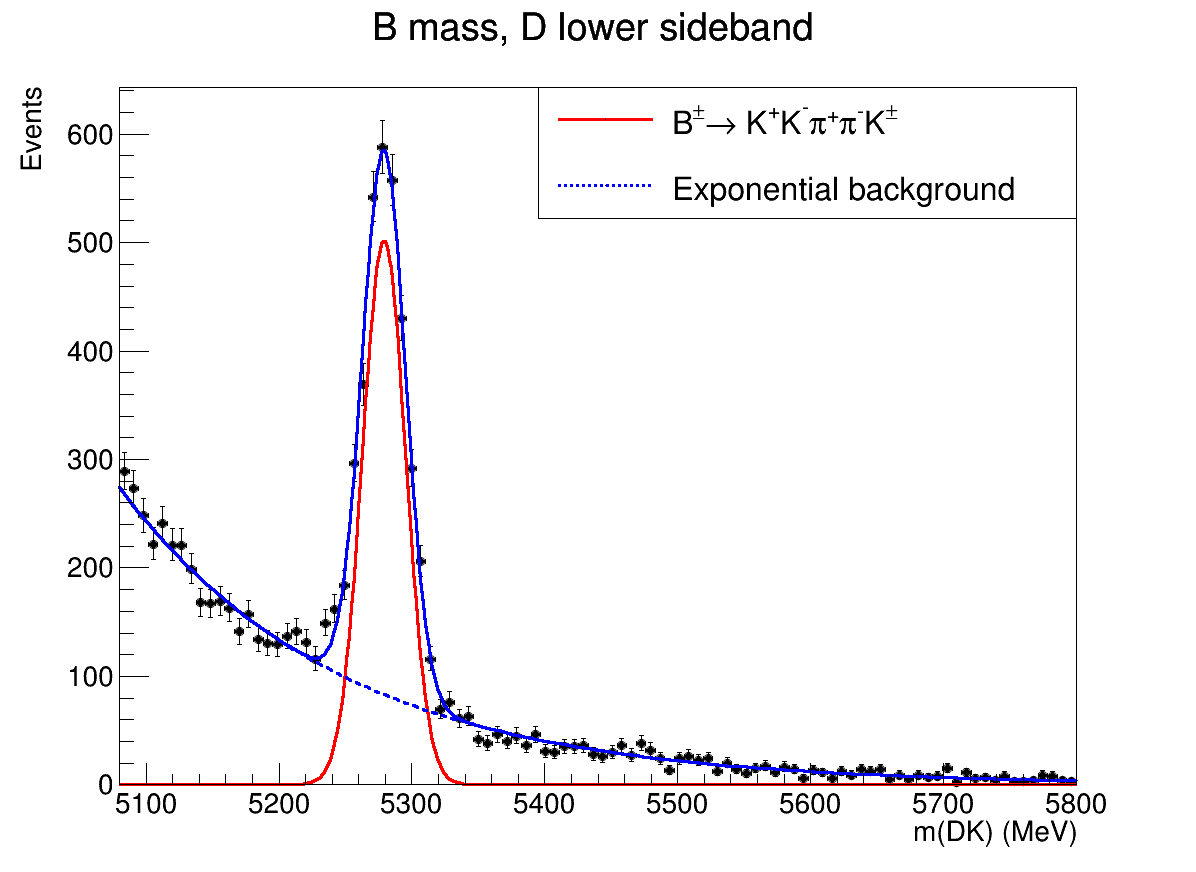
\includegraphics[width = 1.0\textwidth]{B2DKLower_PlusMinus_AllBins_Charmless.png}
      \caption{Without flight significance cut}
    \end{subfigure}%
    \begin{subfigure}{0.5\textwidth}
      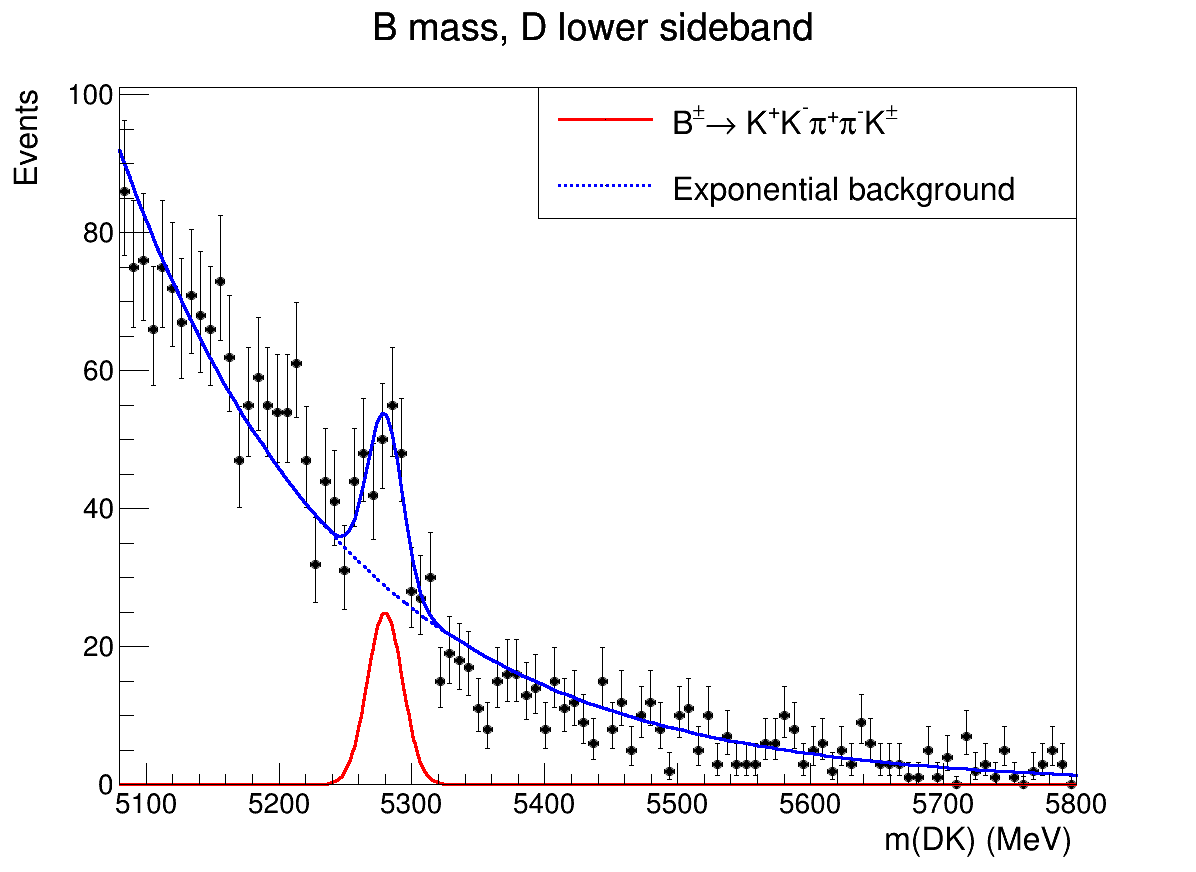
\includegraphics[width = 1.0\textwidth]{B2DKLower_PlusMinus_AllBinsFDCut_Charmless.png}
      \caption{With flight significance cut}
    \end{subfigure}
    \caption{Charmless background in the $D$ sideband}
  \end{figure}
\end{frame}

\begin{frame}{Charmless backgrounds by charge}
  \begin{figure}
    \centering
    \vspace{-0.2cm}
    \begin{subfigure}{0.5\textwidth}
      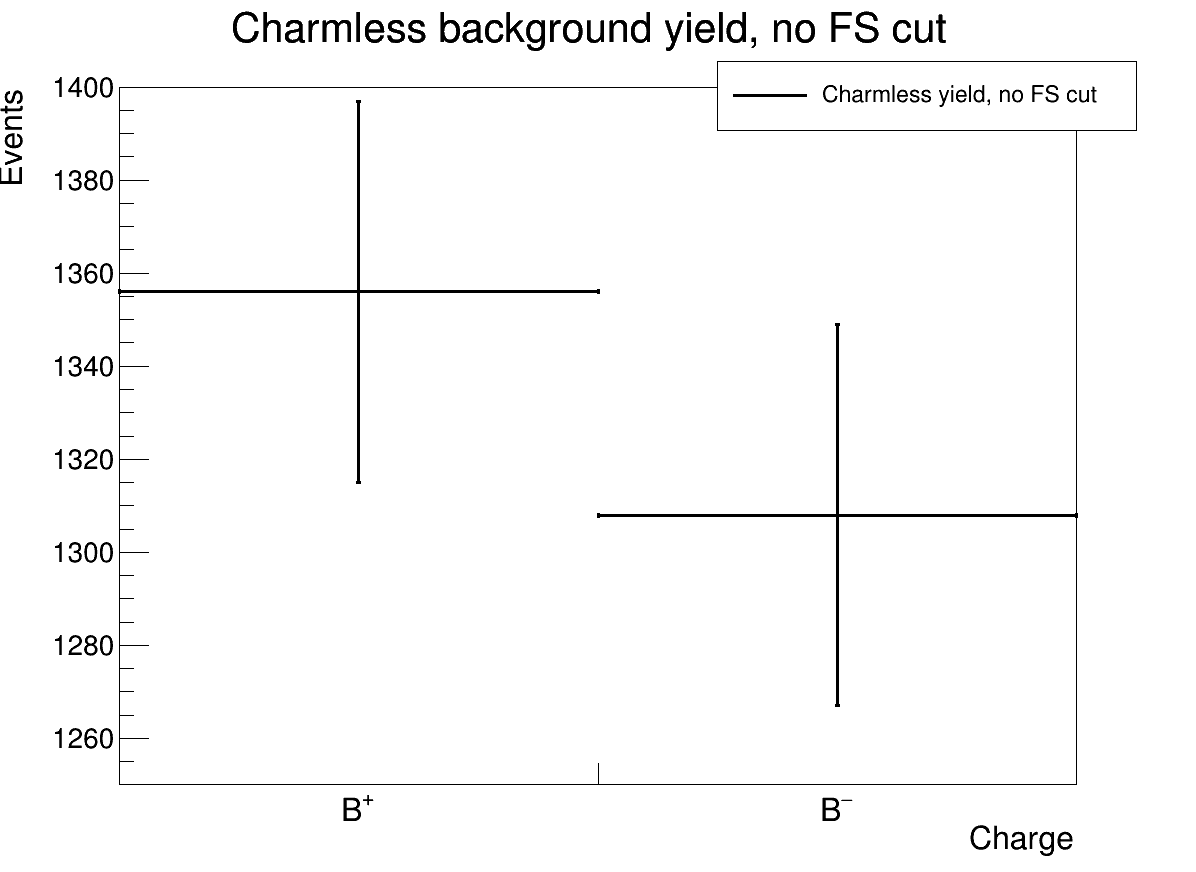
\includegraphics[width = 1.0\textwidth]{CharmlessYieldsCharge.png}
      \caption{Without flight significance cut}
    \end{subfigure}%
    \begin{subfigure}{0.5\textwidth}
      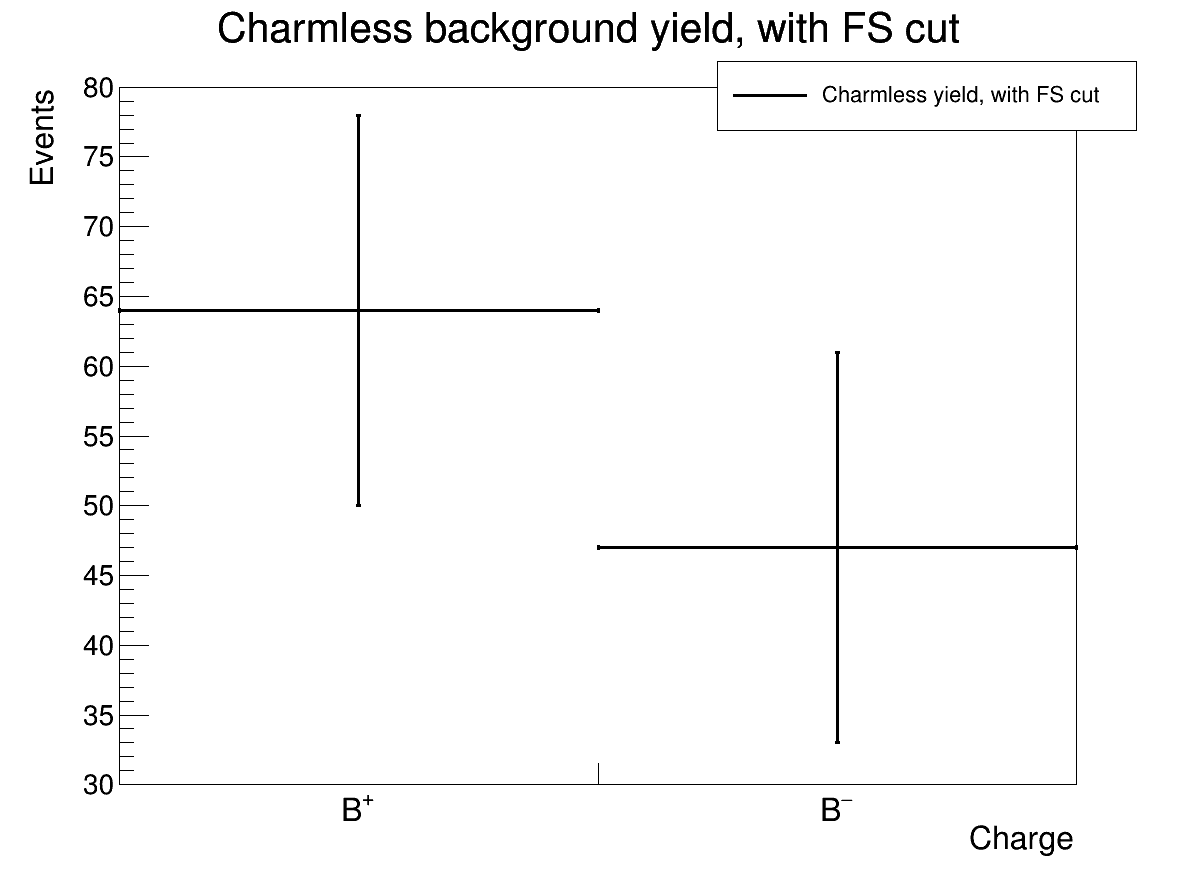
\includegraphics[width = 1.0\textwidth]{CharmlessYieldsFSCutCharge.png}
      \caption{With flight significance cut}
    \end{subfigure}
    \caption{Charmless background split by charge}
  \end{figure}
\end{frame}

\begin{frame}{Charmless backgrounds by bins}
  \begin{figure}
    \centering
    \vspace{-0.2cm}
    \begin{subfigure}{0.5\textwidth}
      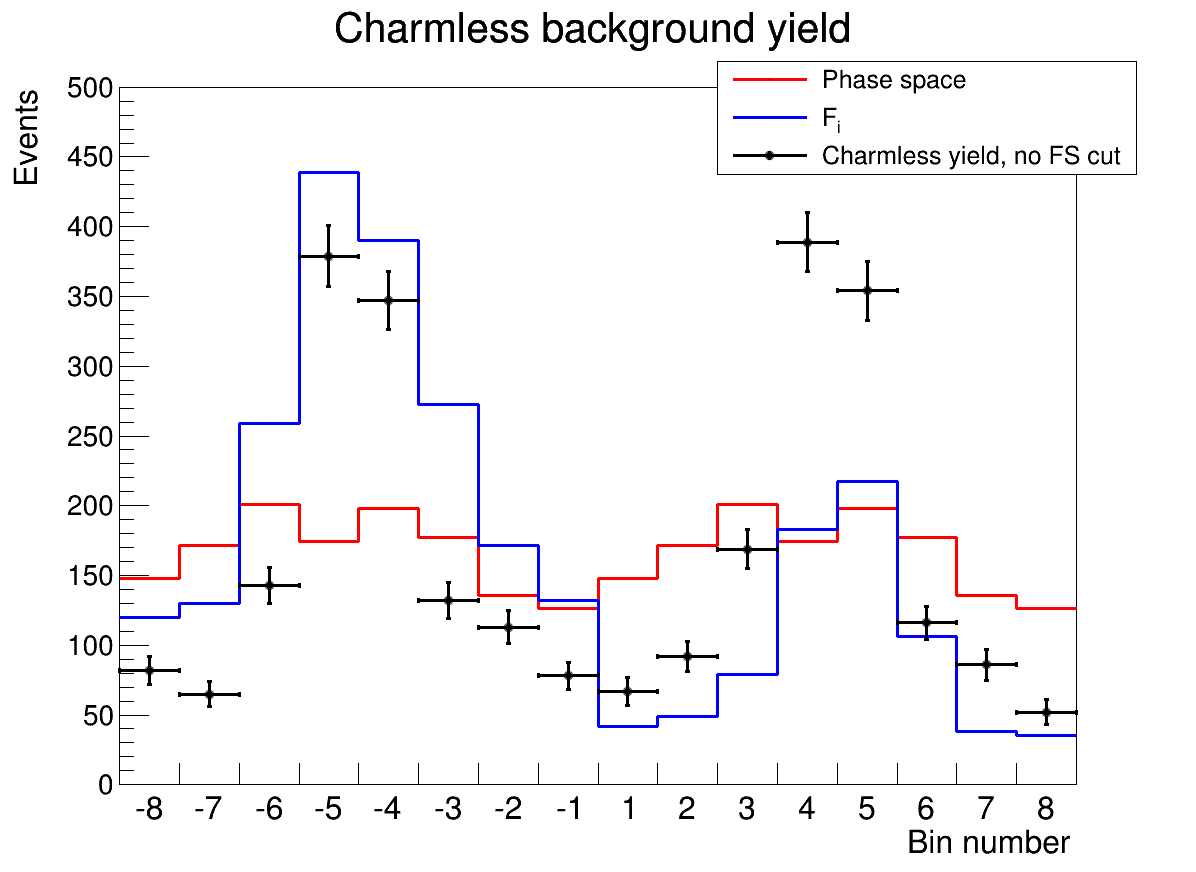
\includegraphics[width = 1.0\textwidth]{CharmlessYieldsBin.png}
      \caption{Without flight significance cut}
    \end{subfigure}%
    \begin{subfigure}{0.5\textwidth}
      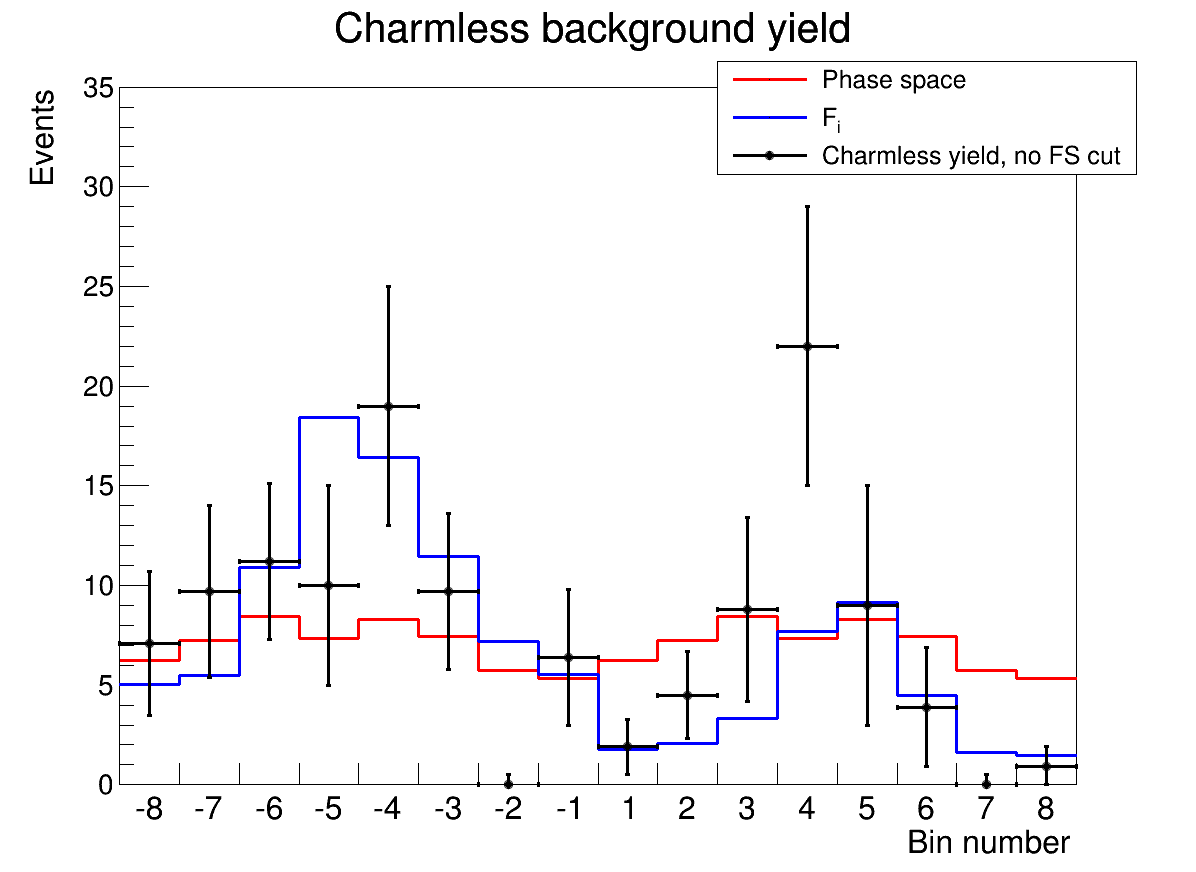
\includegraphics[width = 1.0\textwidth]{CharmlessYieldsFSCutBin.png}
      \caption{With flight significance cut}
    \end{subfigure}
    \caption{Charmless background split by bins}
  \end{figure}
\end{frame}

\begin{frame}{BDT cut optimization}
  \begin{itemize}
    \setlength\itemsep{1.5em}
    \item{Current BDT cut: $0.75$}
    \item{Minimize statistical $\gamma$ error}
    \item{Procedure:}
    \begin{enumerate}
    \setlength\itemsep{0.5em}
      \item{Perform global fit to fix signal and background yields and PDF shapes}
      \item{Generate $1000$ toy datasets using the global fit parameters}
      \item{Fit for $\gamma$}
      \item{Extract expected $\gamma$ precision from $\gamma$ distribution of toy datasets}
    \end{enumerate}
  \end{itemize}
\end{frame}

\begin{frame}{BDT cut optimization}
  \begin{figure}
    \centering
    \vspace{-0.2cm}
    \begin{subfigure}{0.5\textwidth}
      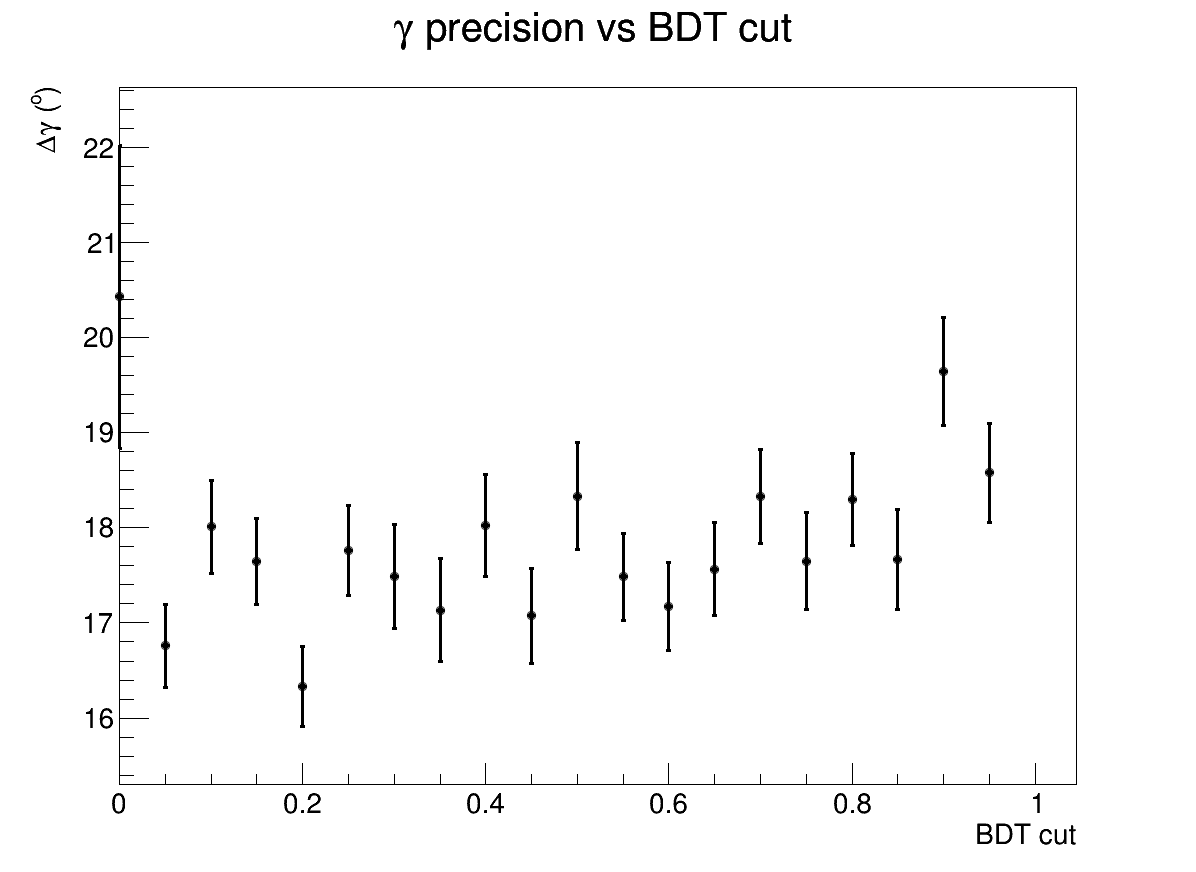
\includegraphics[width = 1.0\textwidth]{BDTOptimization_4Bins_Run2.png}
      \caption{$\gamma$ precision vs BDT cut for $4$ bins}
    \end{subfigure}%
    \begin{subfigure}{0.5\textwidth}
      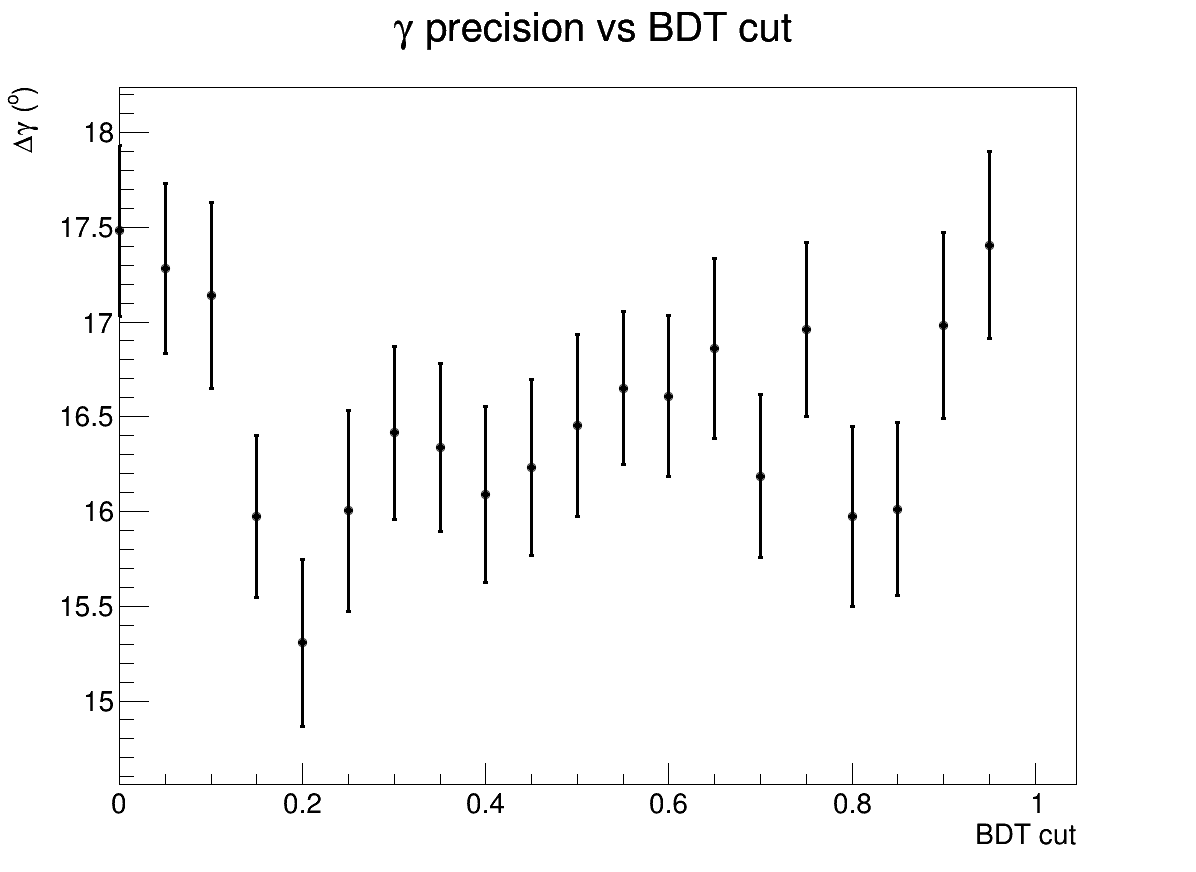
\includegraphics[width = 1.0\textwidth]{BDTOptimization_8Bins_Run2.png}
      \caption{$\gamma$ precision vs BDT cut for $8$ bins}
    \end{subfigure}
  \end{figure}
\end{frame}

\section{Global mass fit}
\begin{frame}{Global mass fit}
  \begin{figure}
    \centering
    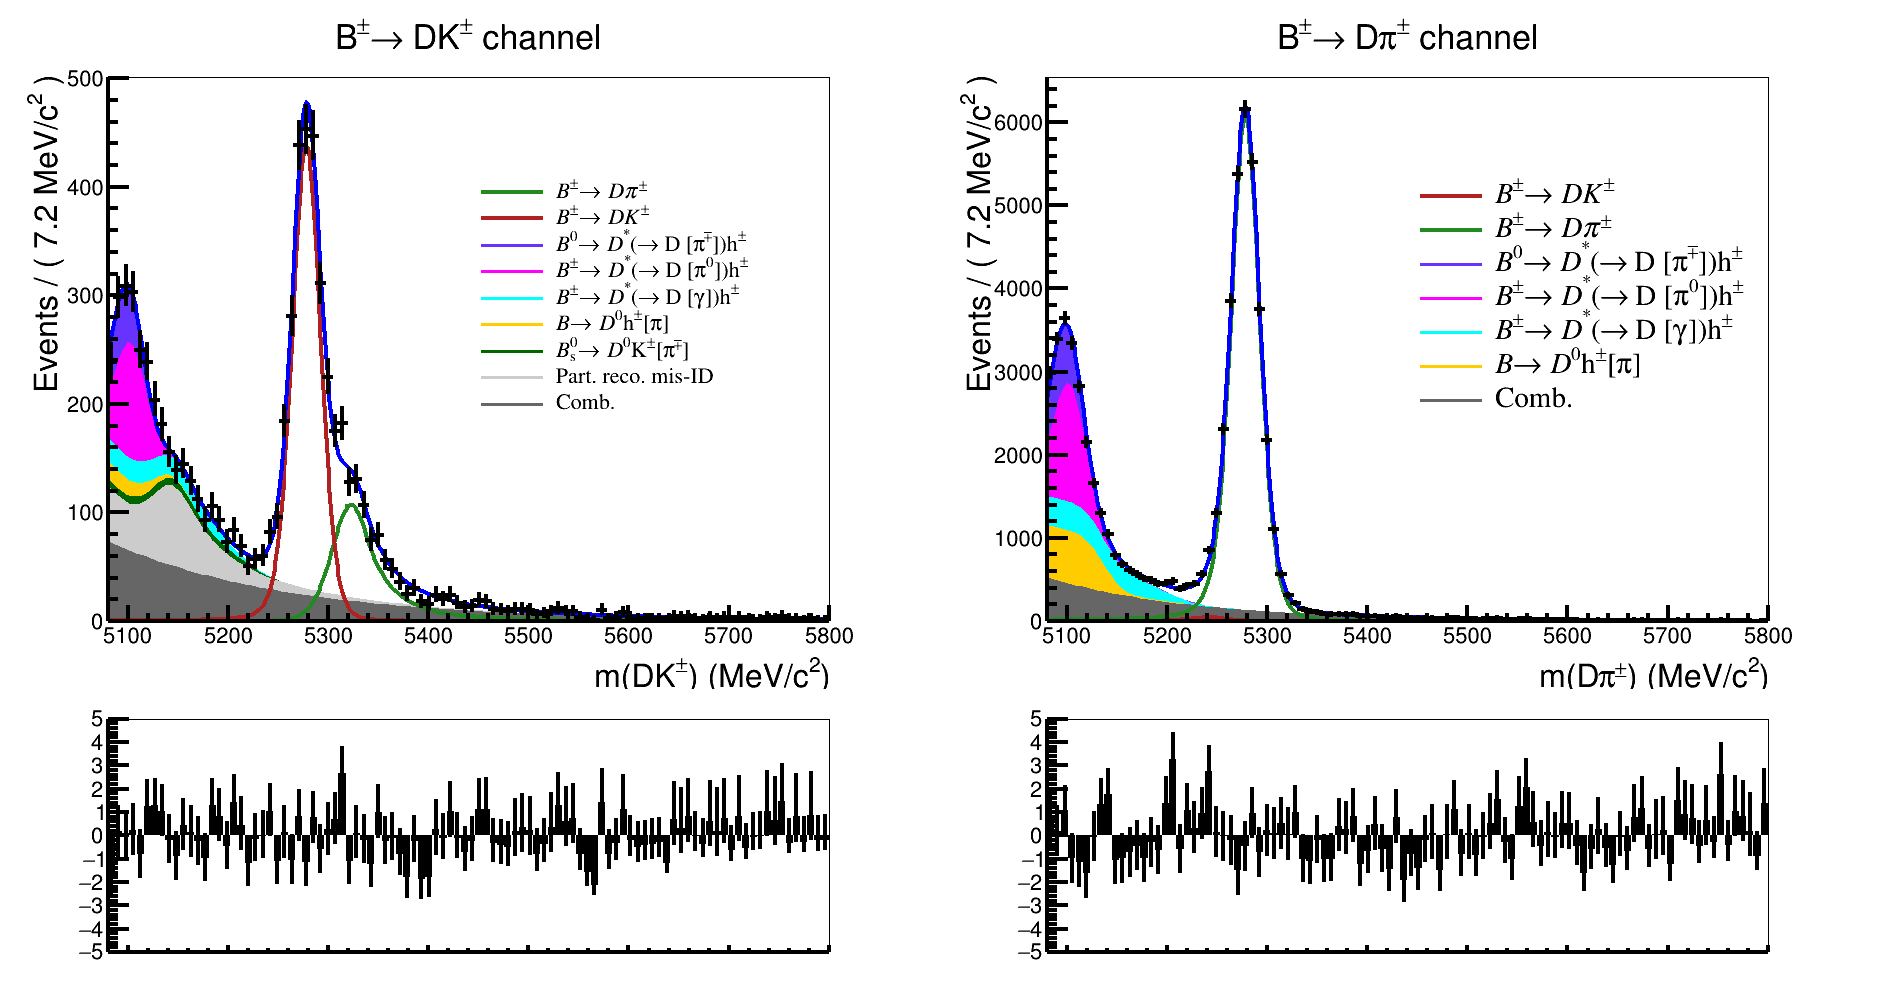
\includegraphics[width = 1.0\textwidth]{GlobalFit.png}
    \caption{Global mass fit (left) $B\to DK$ and (right) $B\to D\pi$}
  \end{figure}
\end{frame}

\section{Toy studies}
\subsection{Standard fits with 4 and 8 bins}
\begin{frame}{Standard toy studies with $4$ bins}
  \begin{figure}
    \centering
    \vspace{-0.2cm}
    \begin{subfigure}{0.5\textwidth}
      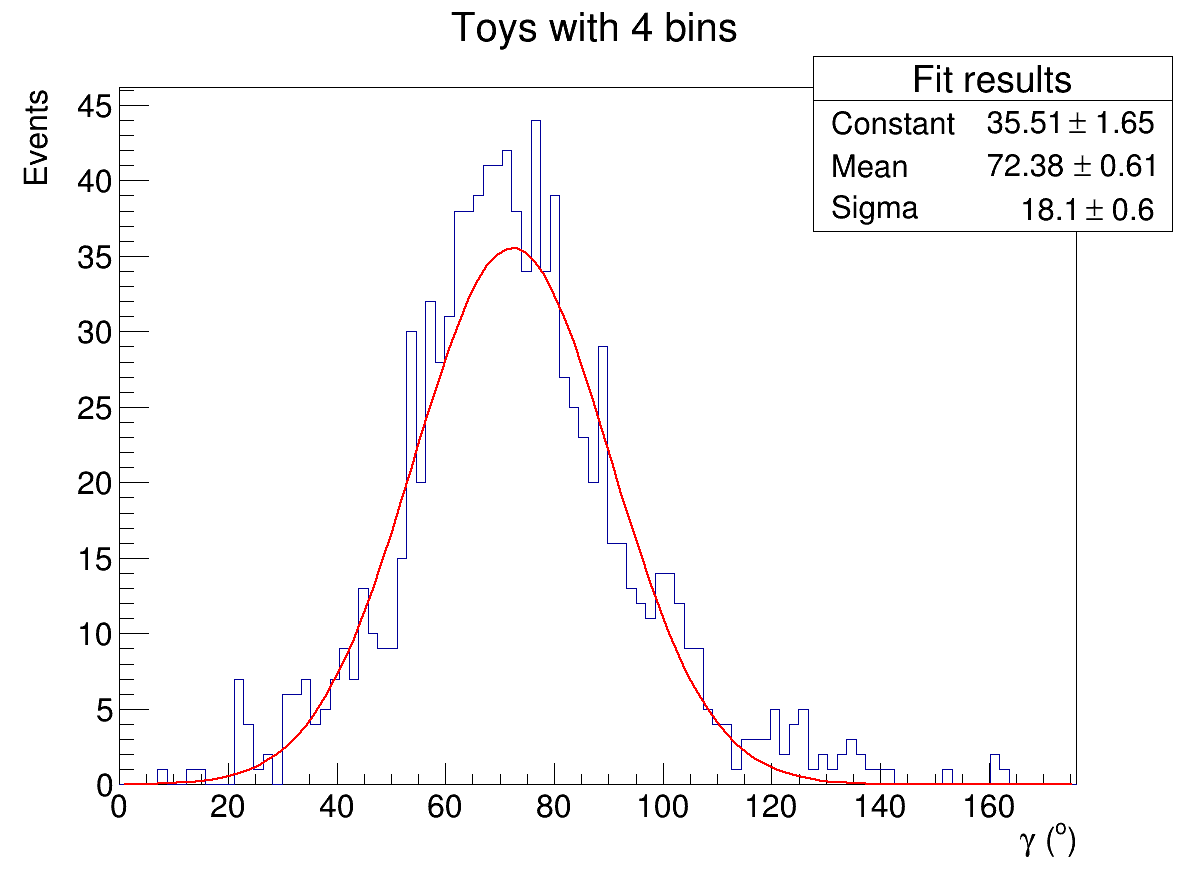
\includegraphics[width = 1.0\textwidth]{Toy_Standard_4Bins.png}
      \caption{$\gamma$ from toys}
    \end{subfigure}%
    \begin{subfigure}{0.5\textwidth}
      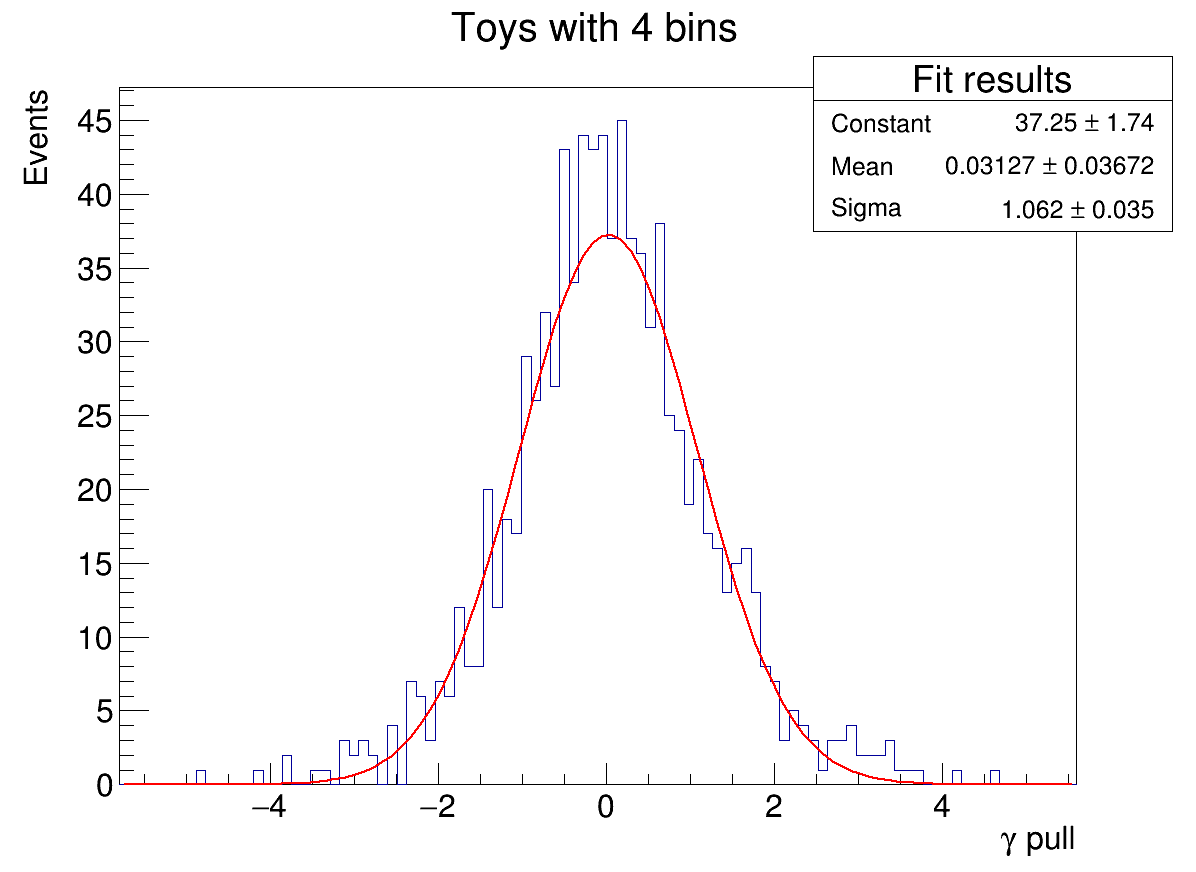
\includegraphics[width = 1.0\textwidth]{Toy_Standard_4Bins_Pull.png}
      \caption{$\gamma$ pull distribution}
    \end{subfigure}
  \end{figure}
\end{frame}

\begin{frame}{Standard toy studies with $8$ bins}
  \begin{figure}
    \centering
    \vspace{-0.2cm}
    \begin{subfigure}{0.5\textwidth}
      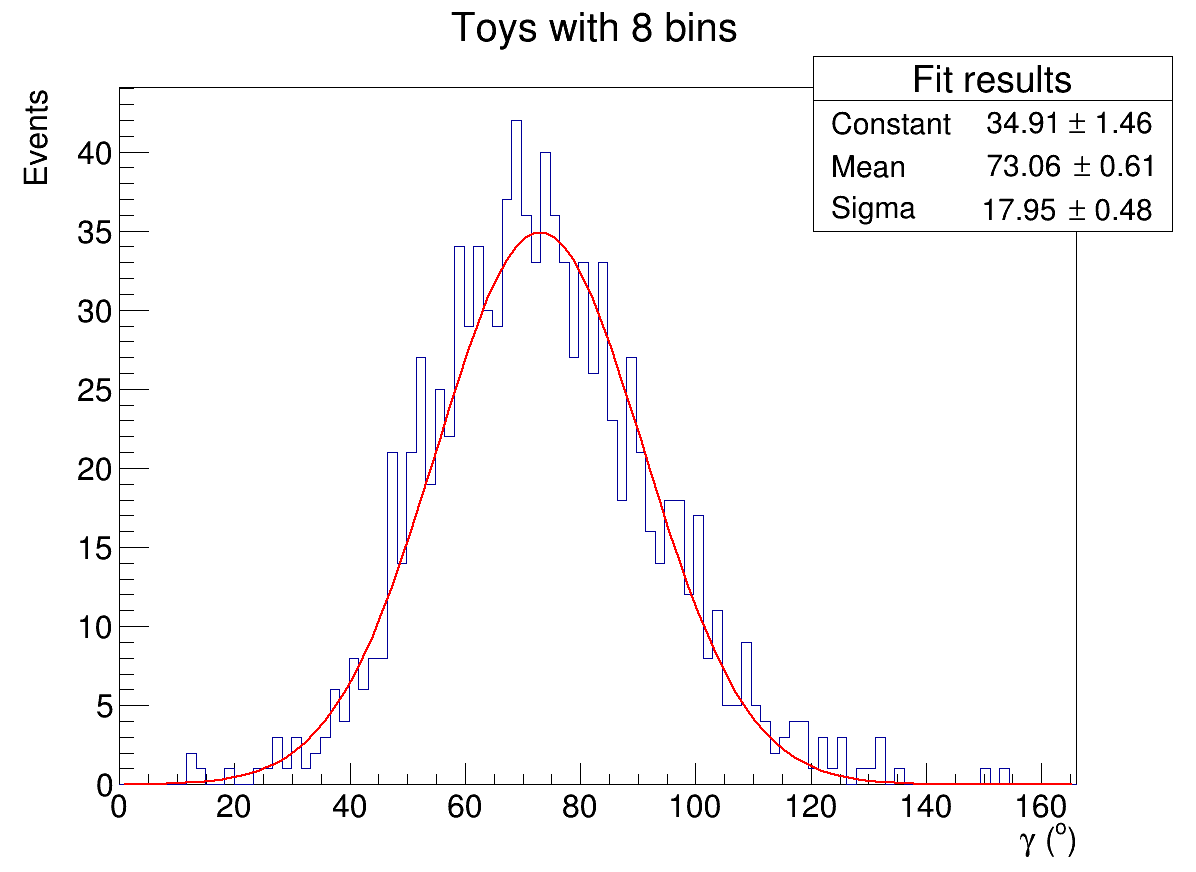
\includegraphics[width = 1.0\textwidth]{Toy_Standard_8Bins.png}
      \caption{$\gamma$ from toys}
    \end{subfigure}%
    \begin{subfigure}{0.5\textwidth}
      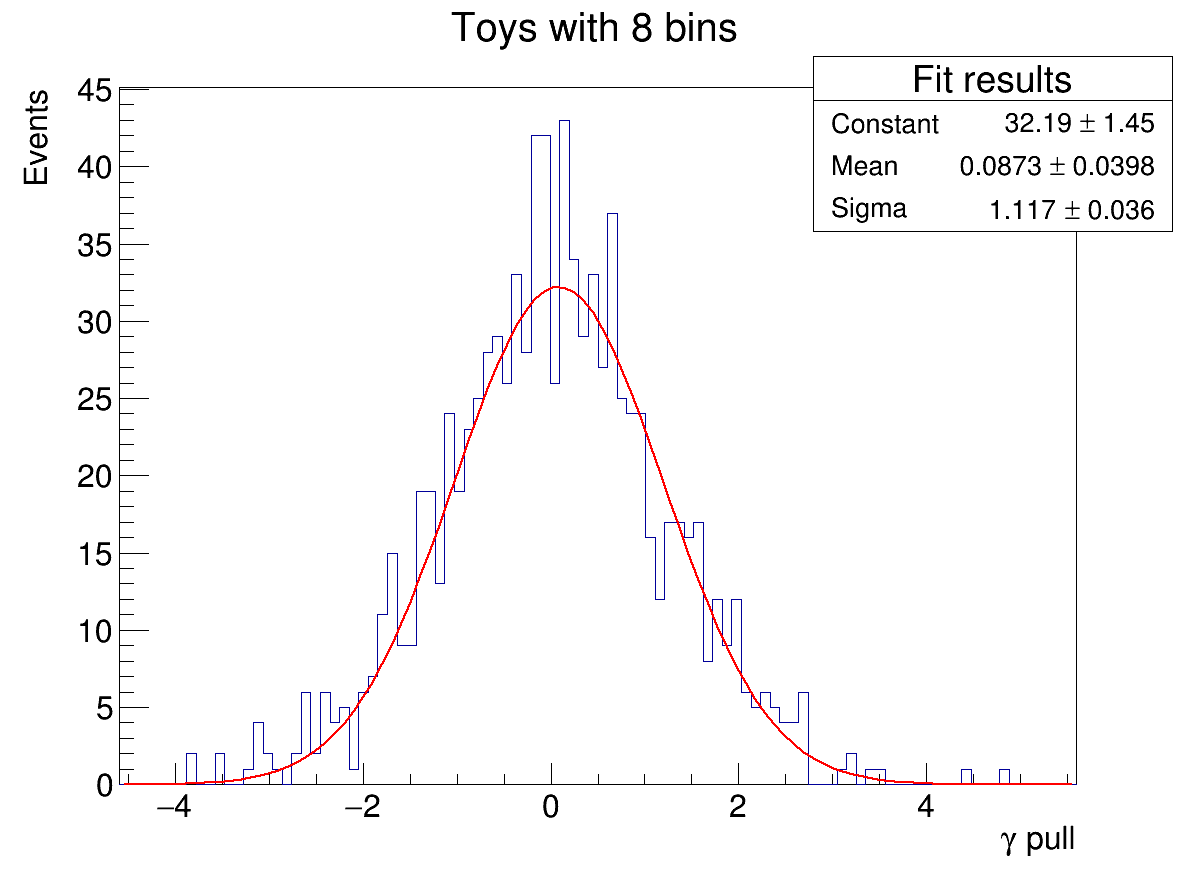
\includegraphics[width = 1.0\textwidth]{Toy_Standard_8Bins_Pull.png}
      \caption{$\gamma$ pull distribution}
    \end{subfigure}
  \end{figure}
\end{frame}

\subsection{Biases in CP observables}
\begin{frame}{Biases in $B\to DK$ CP observables, $4$ bins}
  \begin{figure}
    \centering
    \vspace{-0.2cm}
    \begin{subfigure}{0.42\textwidth}
      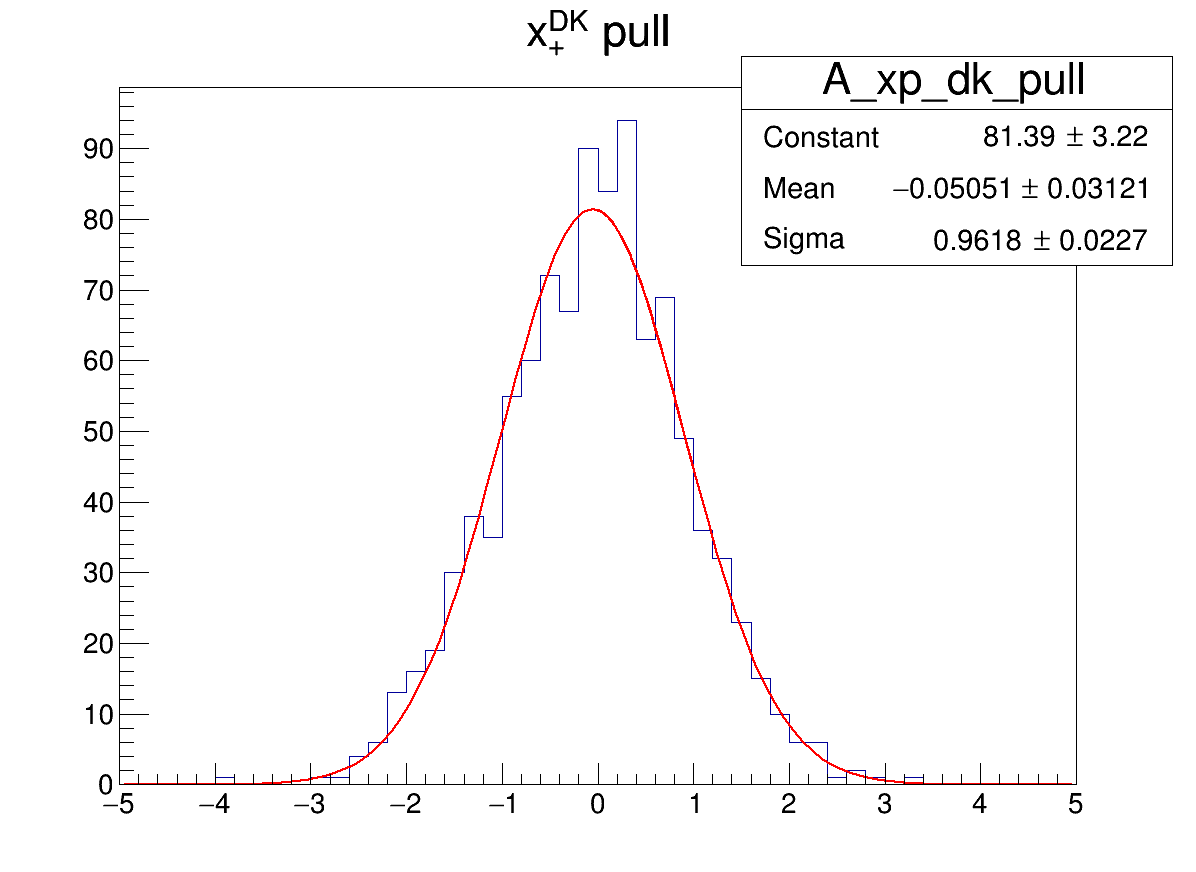
\includegraphics[width = 1.0\textwidth]{A_xp_dk_4Bins_pull.png}
    \end{subfigure}%
    \begin{subfigure}{0.42\textwidth}
      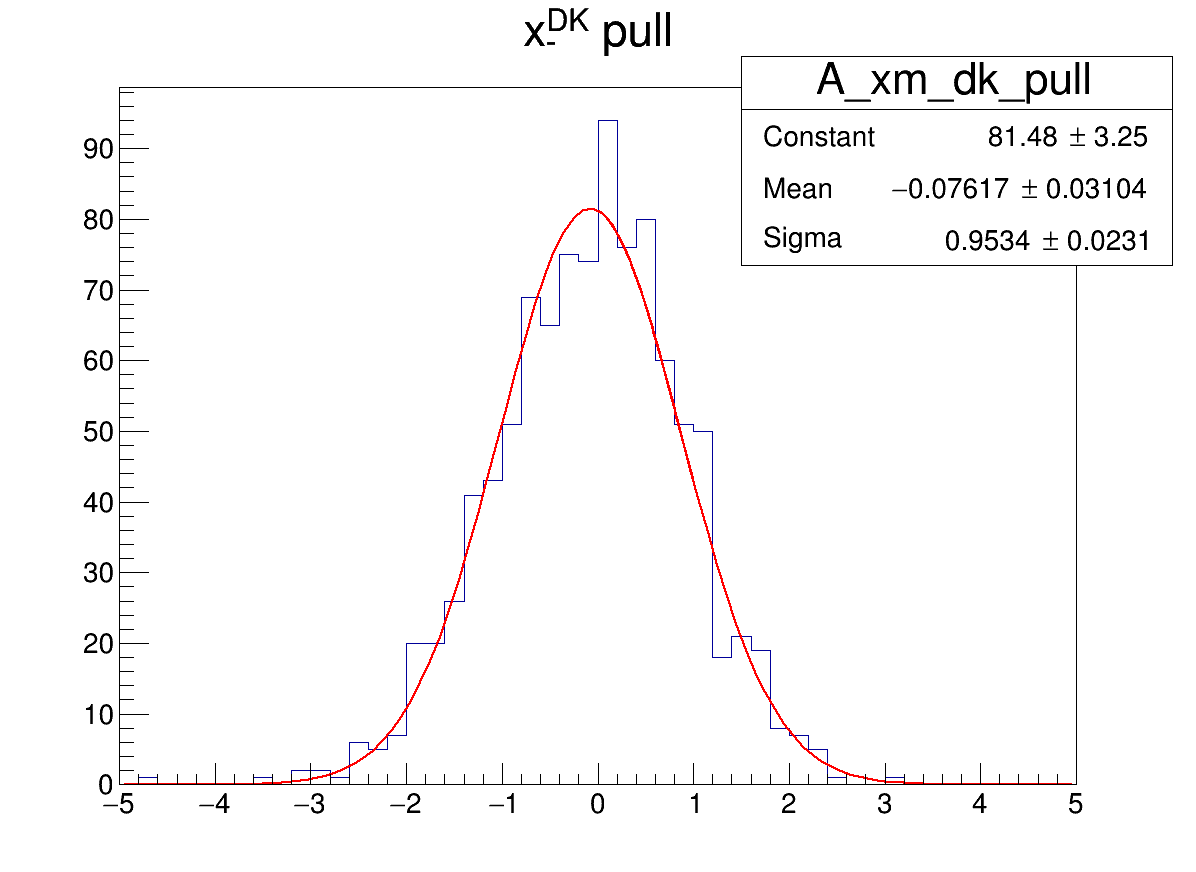
\includegraphics[width = 1.0\textwidth]{A_xm_dk_4Bins_pull.png}
    \end{subfigure}
    \begin{subfigure}{0.42\textwidth}
      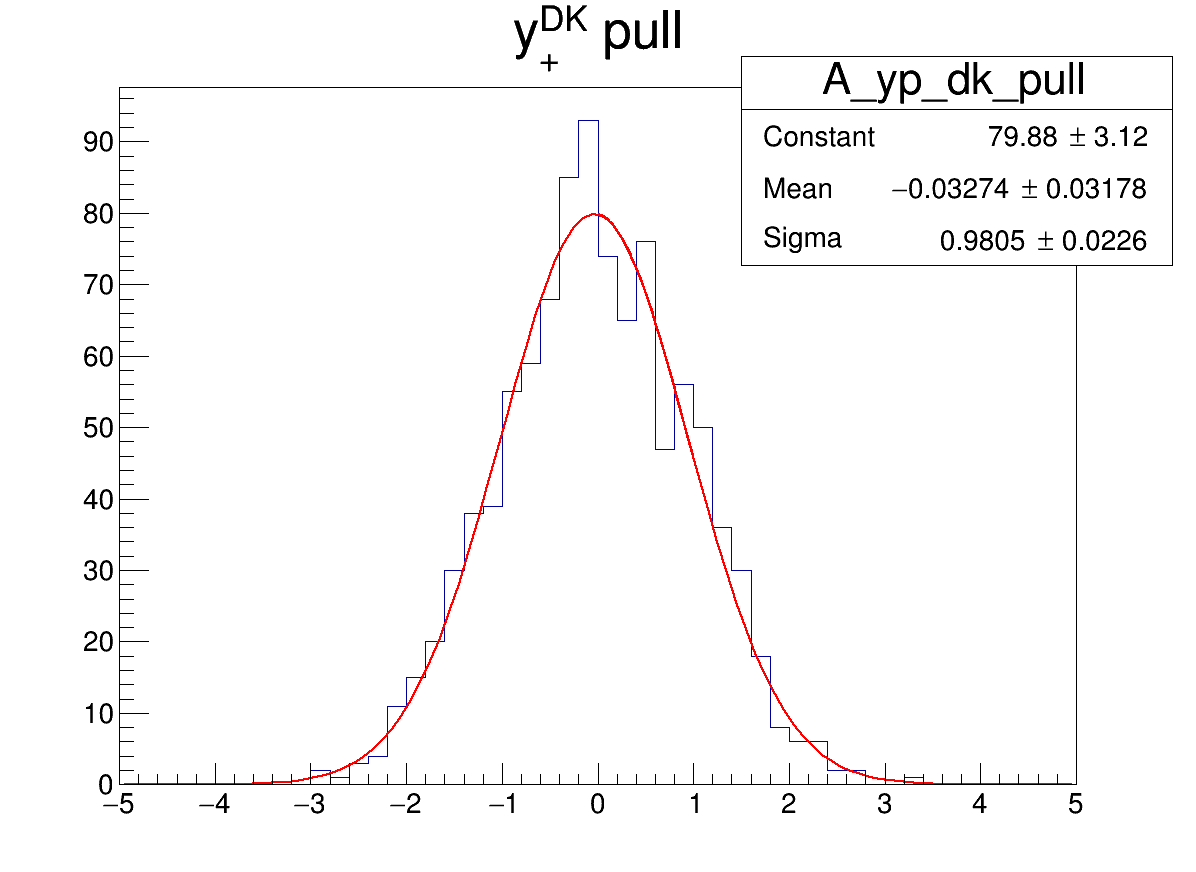
\includegraphics[width = 1.0\textwidth]{A_yp_dk_4Bins_pull.png}
    \end{subfigure}%
    \begin{subfigure}{0.42\textwidth}
      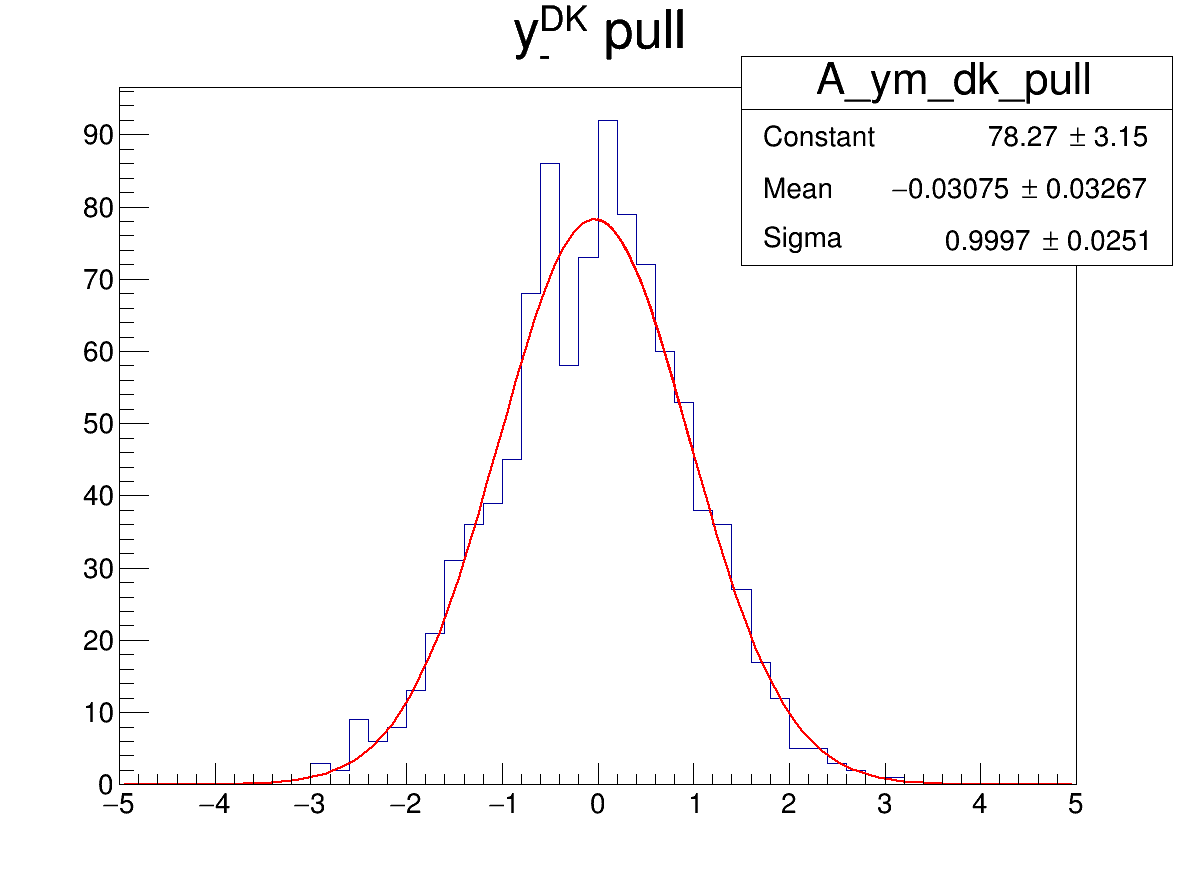
\includegraphics[width = 1.0\textwidth]{A_ym_dk_4Bins_pull.png}
    \end{subfigure}
    \caption{$B\to DK$ CP observable pull distributions}
  \end{figure}
\end{frame}

\begin{frame}{Biases in $B\to DK$ CP observables, $8$ bins}
  \begin{figure}
    \centering
    \vspace{-0.2cm}
    \begin{subfigure}{0.42\textwidth}
      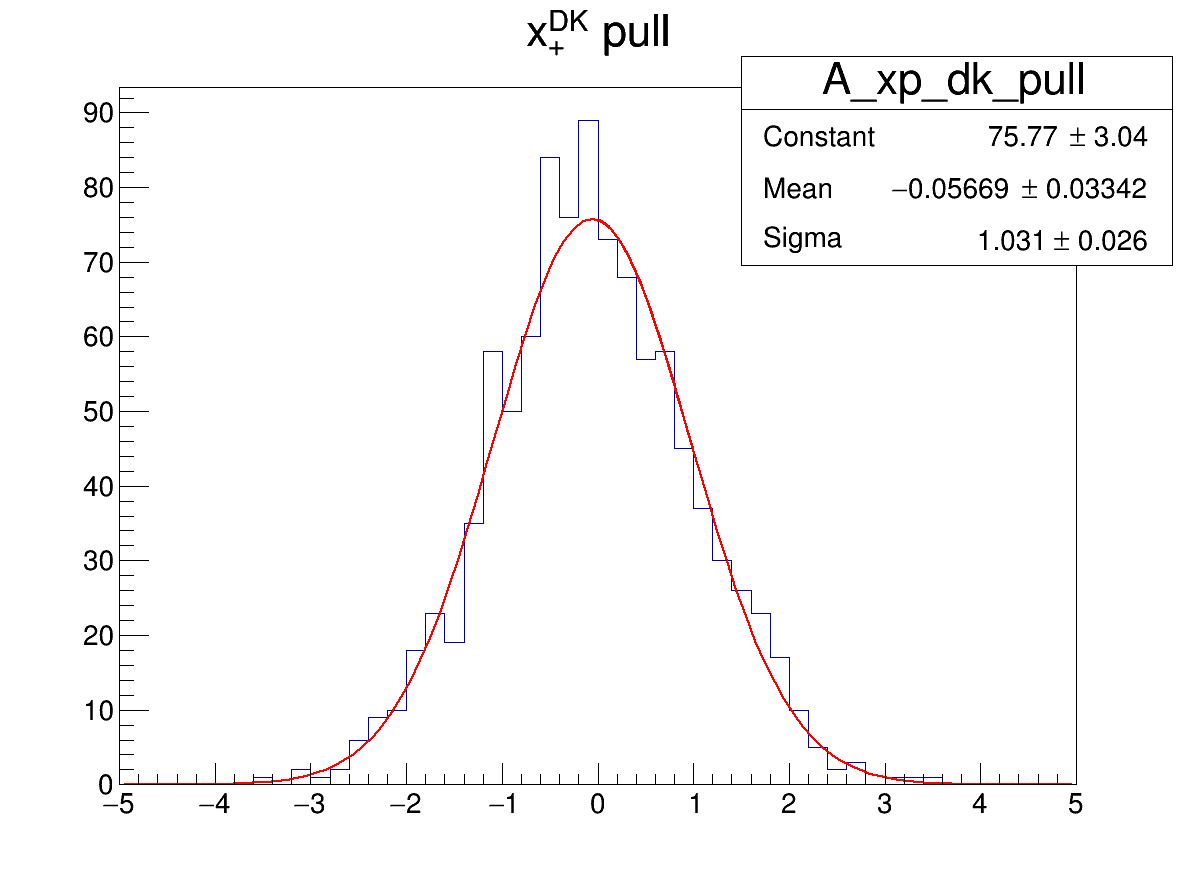
\includegraphics[width = 1.0\textwidth]{A_xp_dk_8Bins_pull.png}
    \end{subfigure}%
    \begin{subfigure}{0.42\textwidth}
      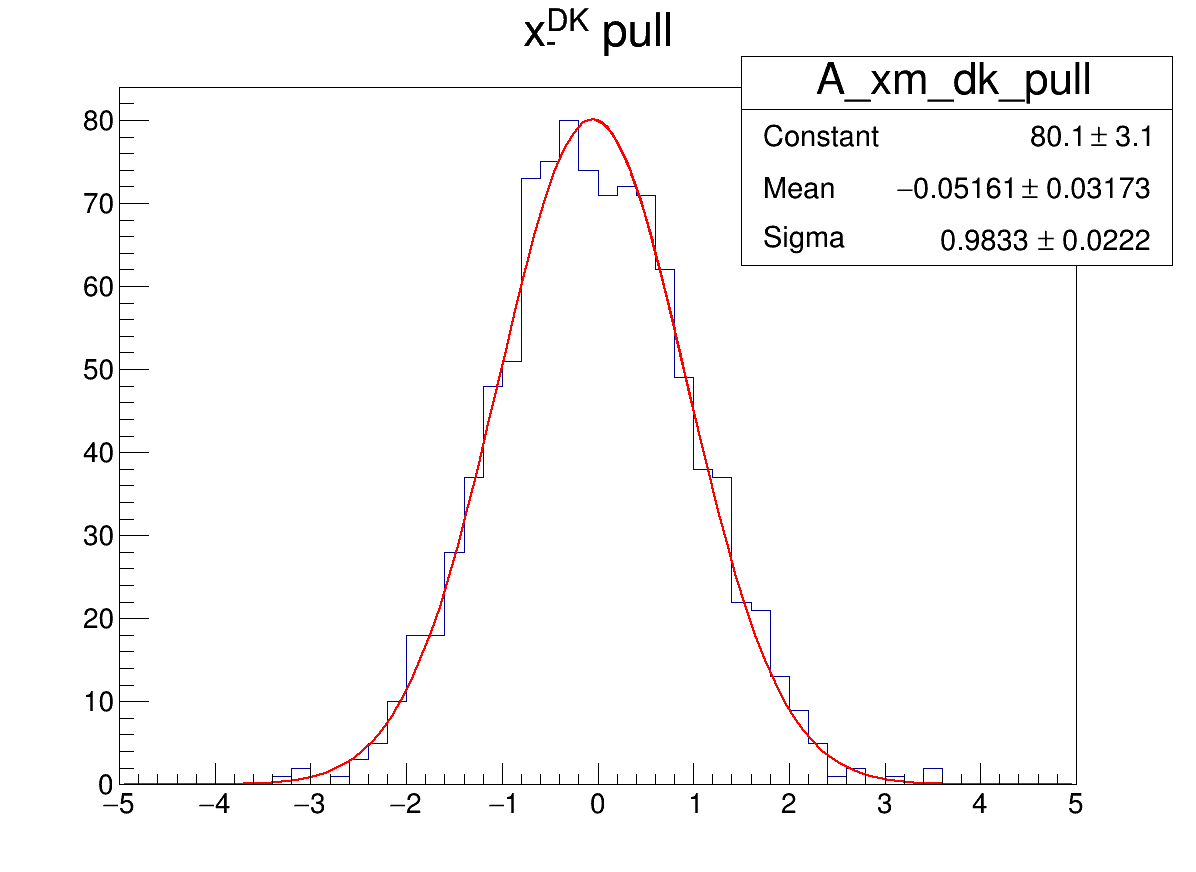
\includegraphics[width = 1.0\textwidth]{A_xm_dk_8Bins_pull.png}
    \end{subfigure}
    \begin{subfigure}{0.42\textwidth}
      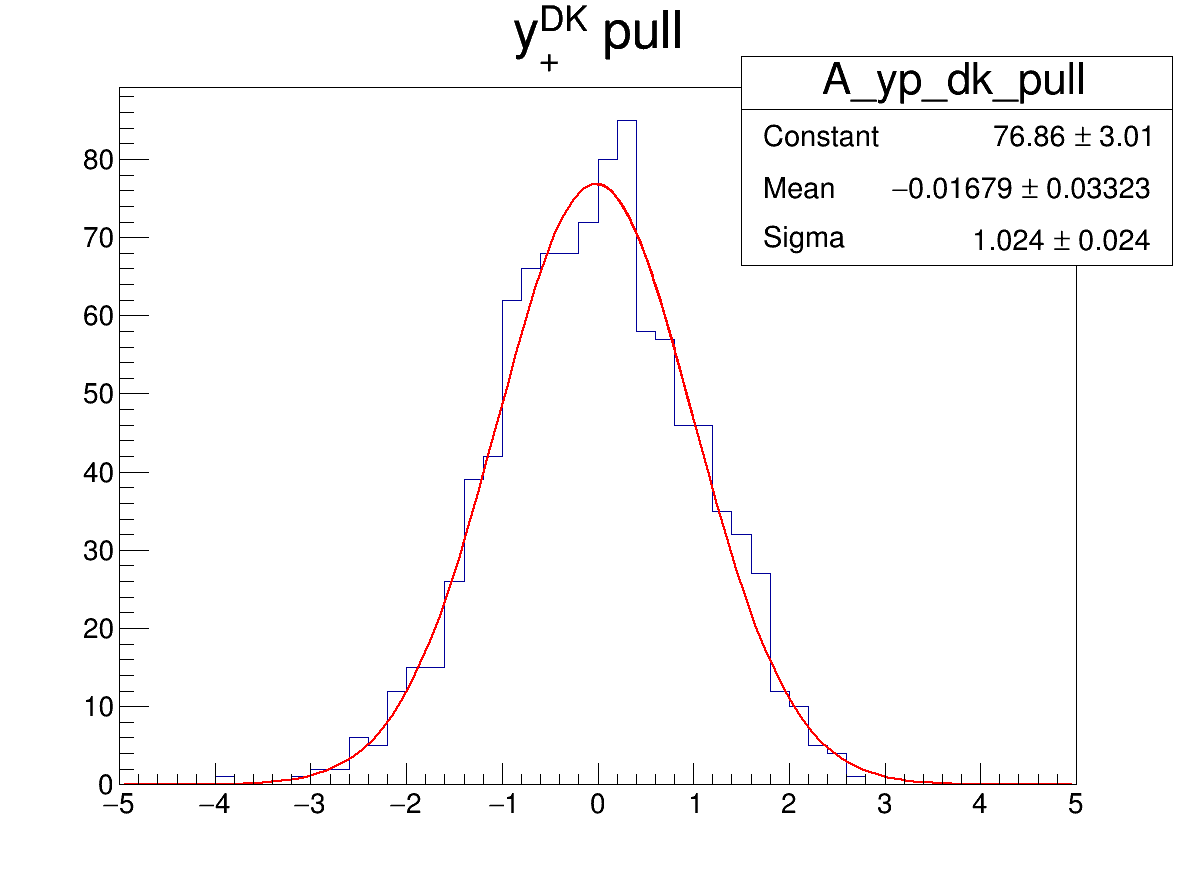
\includegraphics[width = 1.0\textwidth]{A_yp_dk_8Bins_pull.png}
    \end{subfigure}%
    \begin{subfigure}{0.42\textwidth}
      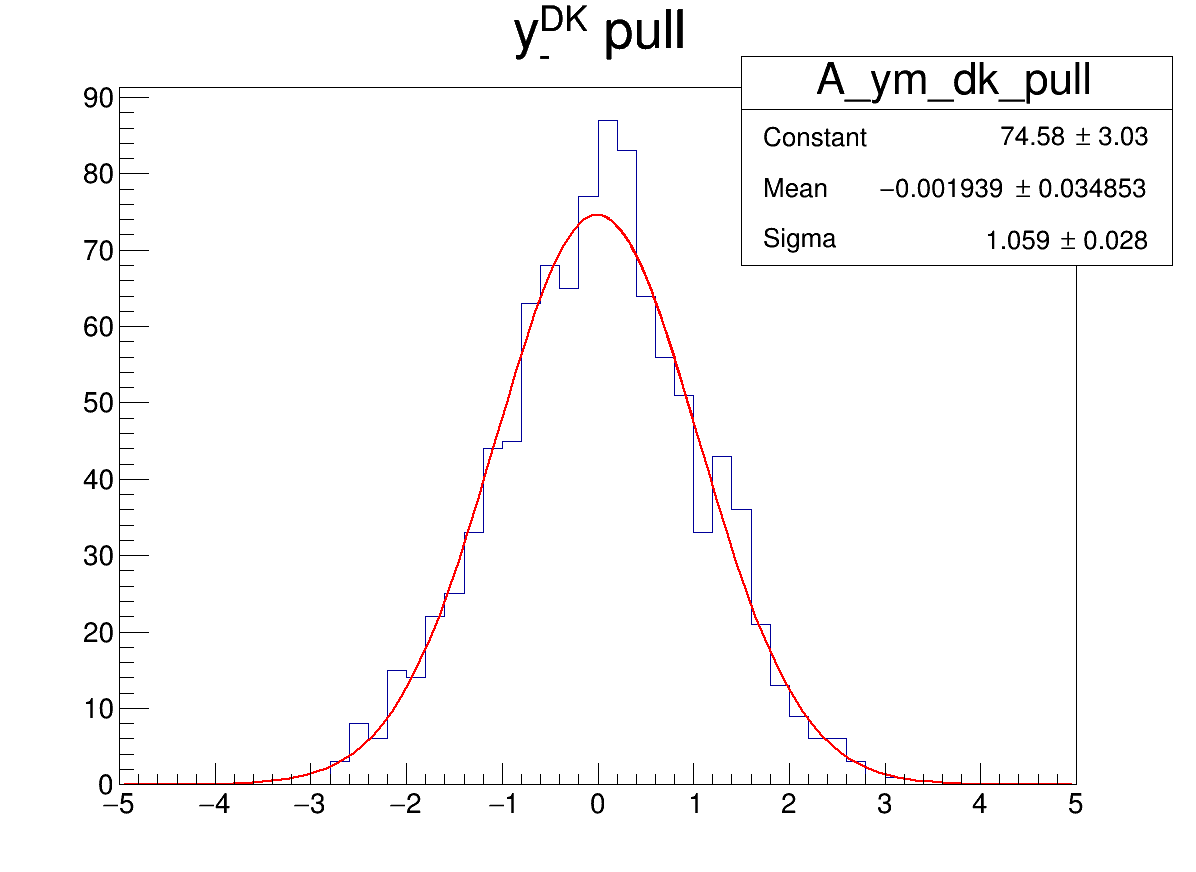
\includegraphics[width = 1.0\textwidth]{A_ym_dk_8Bins_pull.png}
    \end{subfigure}
    \caption{$B\to DK$ CP observable pull distributions}
  \end{figure}
\end{frame}

\begin{frame}{Biases in $B\to D\pi$ CP observables, $4$ bins}
  \begin{figure}
    \centering
    \vspace{-0.2cm}
    \begin{subfigure}{0.5\textwidth}
      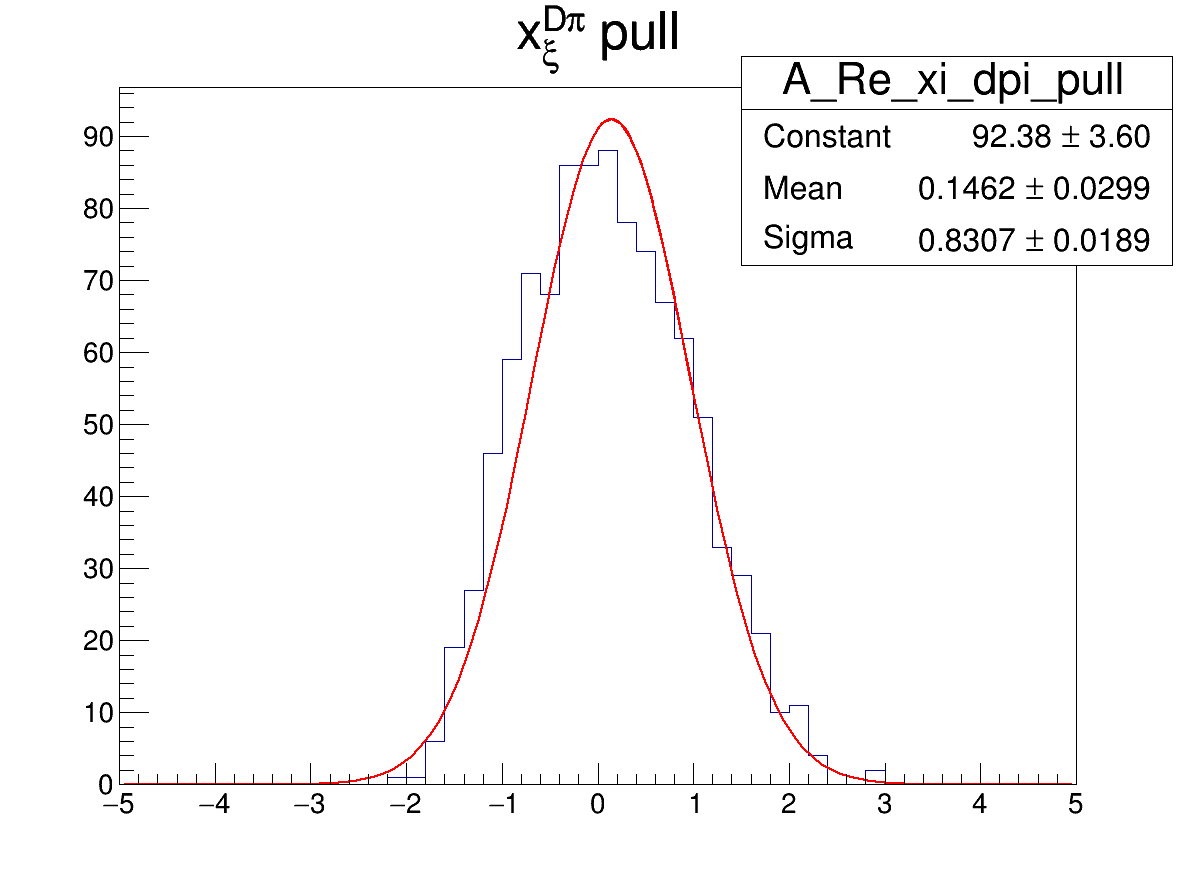
\includegraphics[width = 1.0\textwidth]{A_Re_xi_dpi_4Bins_pull.png}
    \end{subfigure}%
    \begin{subfigure}{0.5\textwidth}
      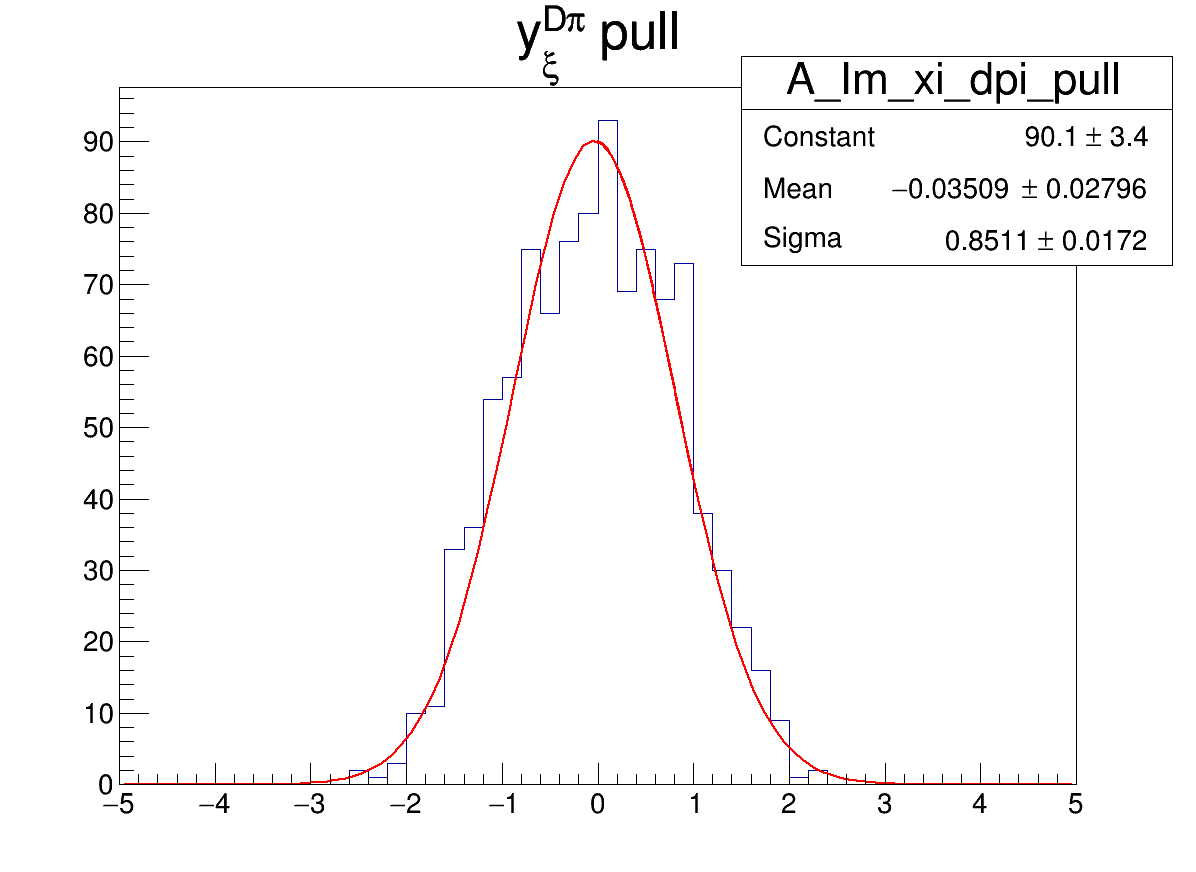
\includegraphics[width = 1.0\textwidth]{A_Im_xi_dpi_4Bins_pull.png}
    \end{subfigure}
    \caption{$B\to D\pi$ CP observable pull distributions}
  \end{figure}
\end{frame}

\begin{frame}{Biases in $B\to D\pi$ CP observables, $4$ bins, $2$x statistics}
  \begin{figure}
    \centering
    \vspace{-0.2cm}
    \begin{subfigure}{0.5\textwidth}
      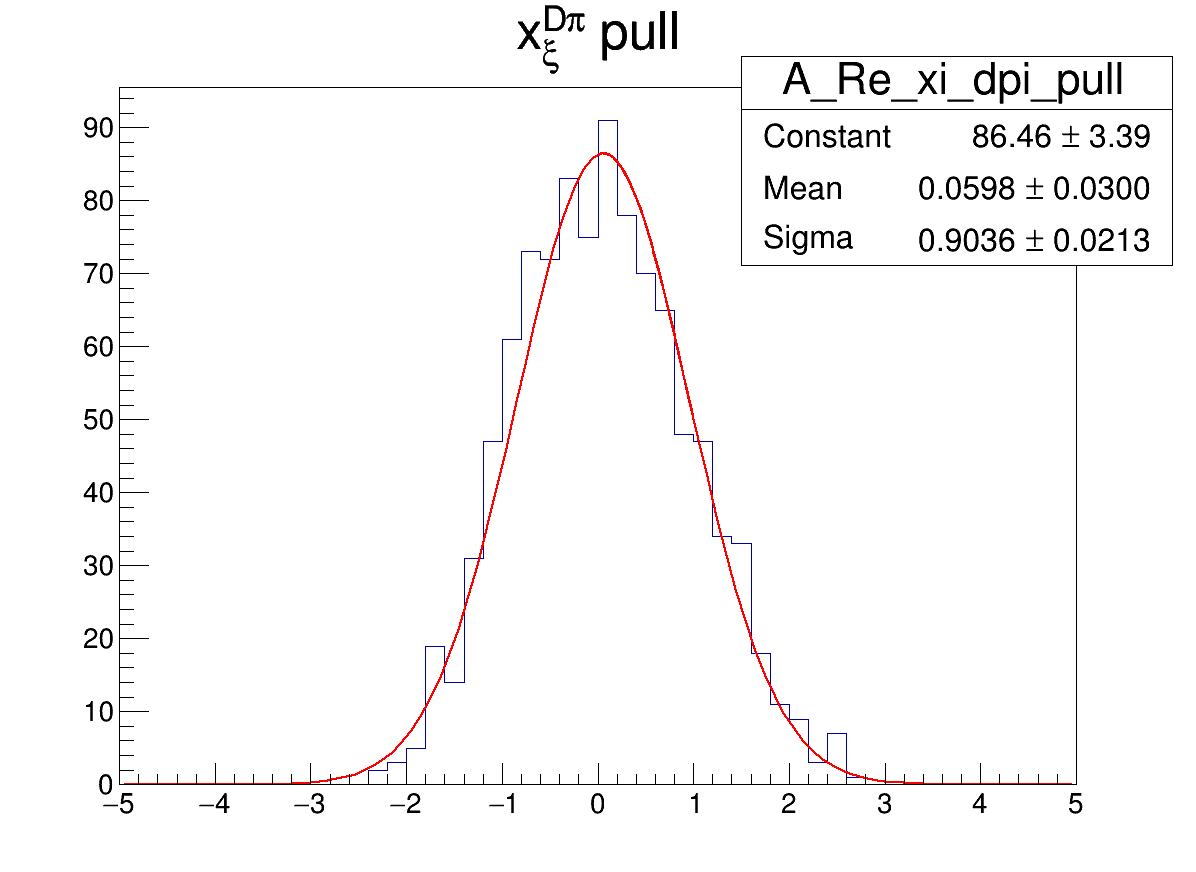
\includegraphics[width = 1.0\textwidth]{A_Re_xi_dpi_4Bins_StatsMultiplier2_pull.png}
    \end{subfigure}%
    \begin{subfigure}{0.5\textwidth}
      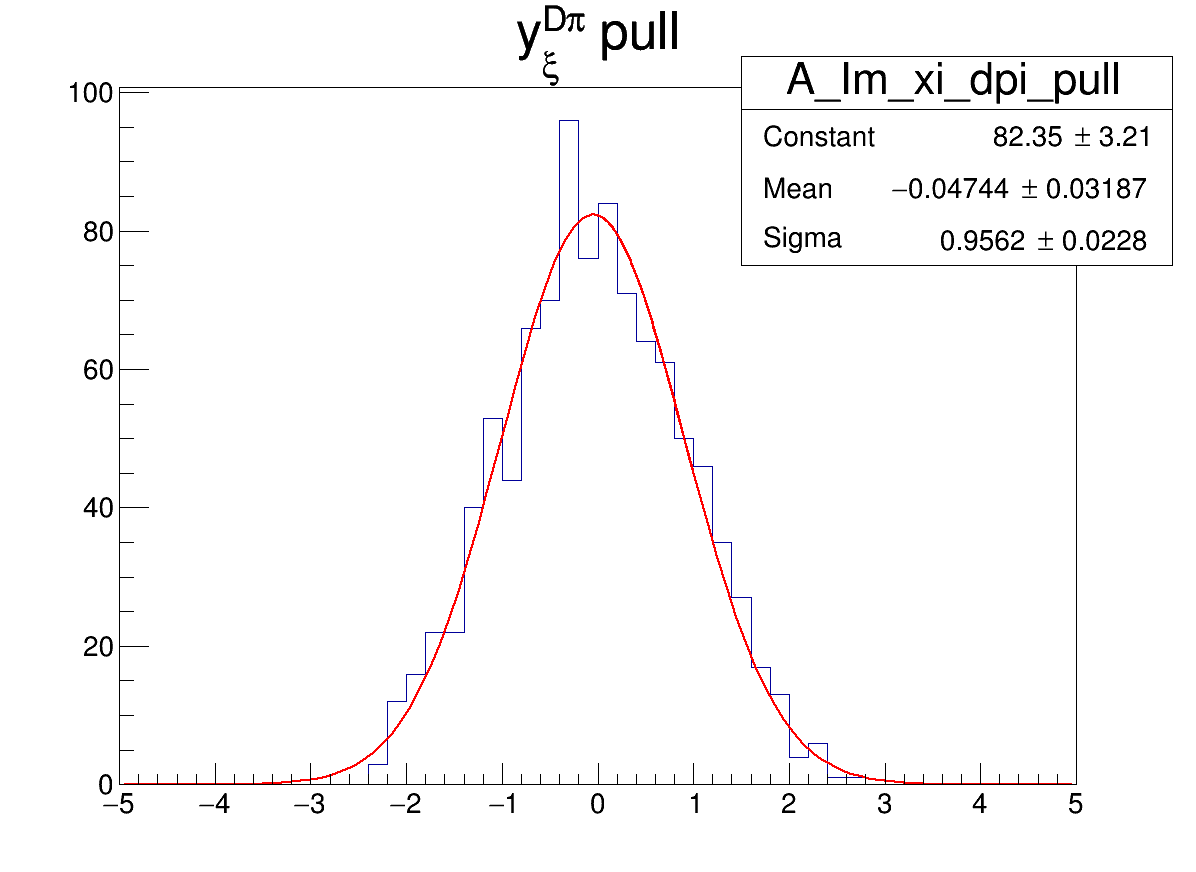
\includegraphics[width = 1.0\textwidth]{A_Im_xi_dpi_4Bins_StatsMultiplier2_pull.png}
    \end{subfigure}
    \caption{$B\to D\pi$ CP observable pull distributions}
  \end{figure}
\end{frame}

\begin{frame}{Biases in $B\to D\pi$ CP observables, $4$ bins, $10$x statistics}
  \begin{figure}
    \centering
    \vspace{-0.2cm}
    \begin{subfigure}{0.5\textwidth}
      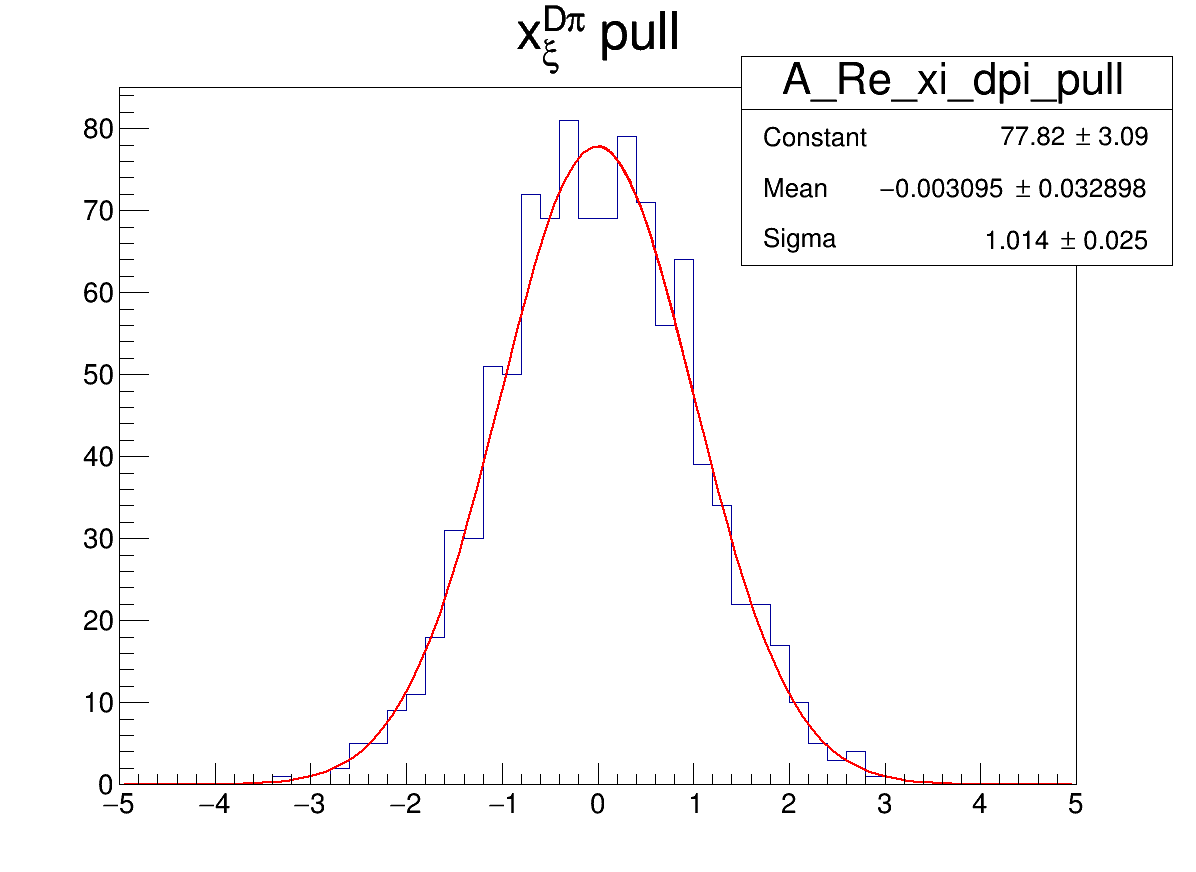
\includegraphics[width = 1.0\textwidth]{A_Re_xi_dpi_4Bins_StatsMultiplier10_pull.png}
    \end{subfigure}%
    \begin{subfigure}{0.5\textwidth}
      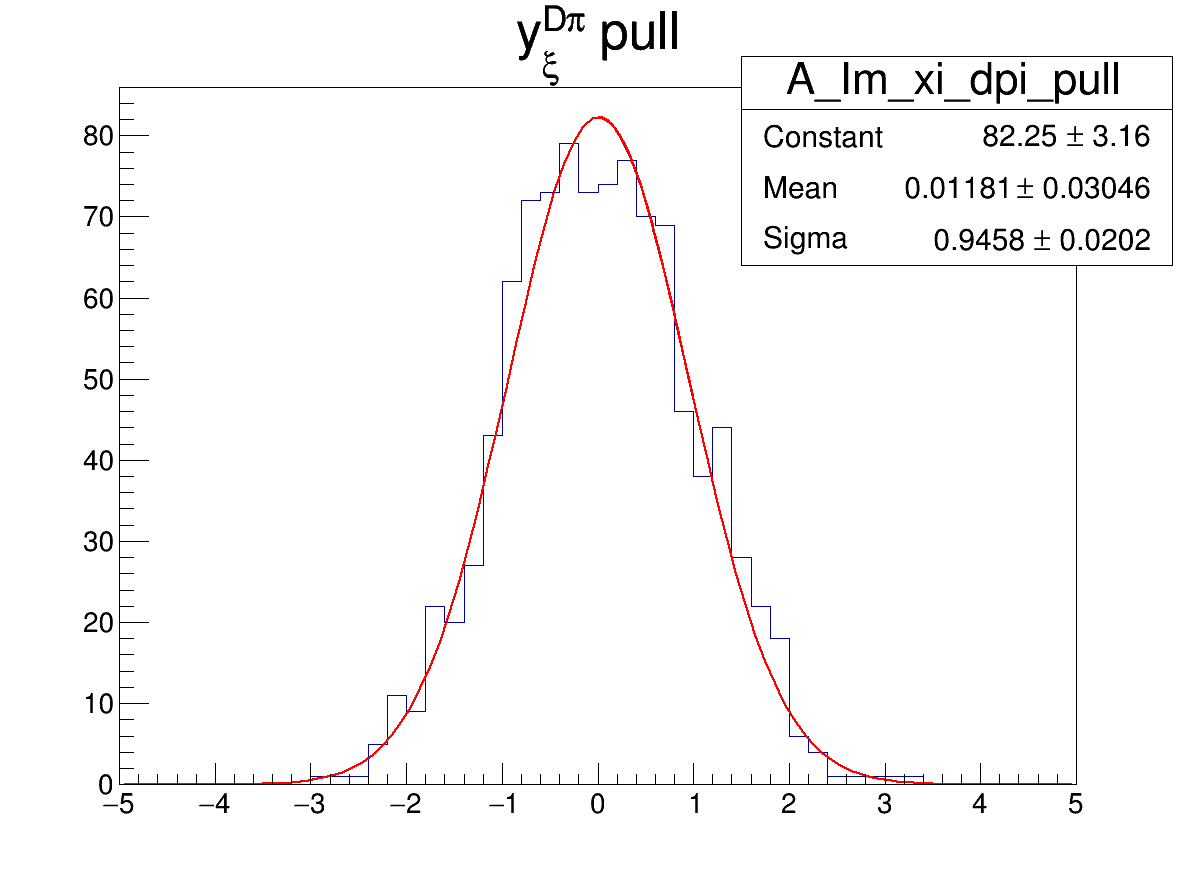
\includegraphics[width = 1.0\textwidth]{A_Im_xi_dpi_4Bins_StatsMultiplier10_pull.png}
    \end{subfigure}
    \caption{$B\to D\pi$ CP observable pull distributions}
  \end{figure}
\end{frame}

\begin{frame}{Biases in $B\to D\pi$ CP observables, $8$ bins}
  \begin{figure}
    \centering
    \vspace{-0.2cm}
    \begin{subfigure}{0.5\textwidth}
      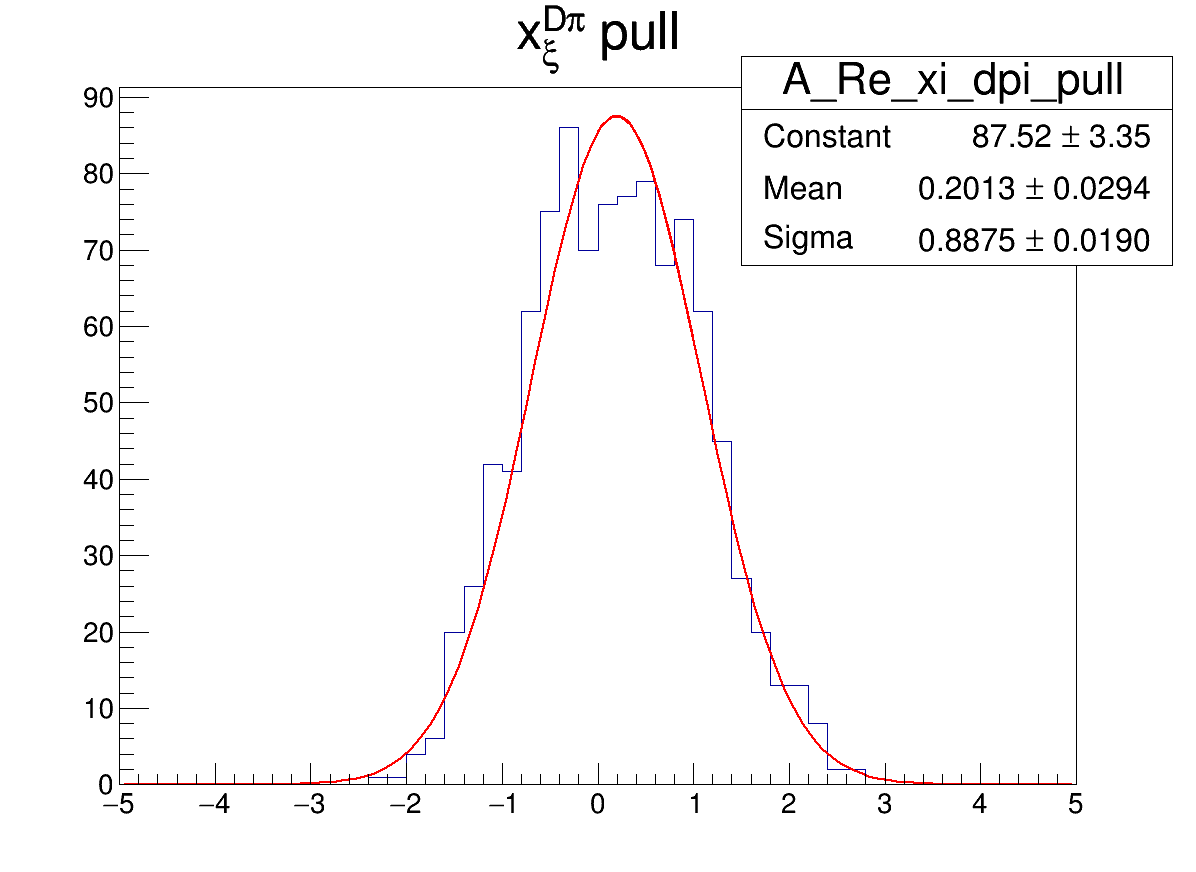
\includegraphics[width = 1.0\textwidth]{A_Re_xi_dpi_8Bins_pull.png}
    \end{subfigure}%
    \begin{subfigure}{0.5\textwidth}
      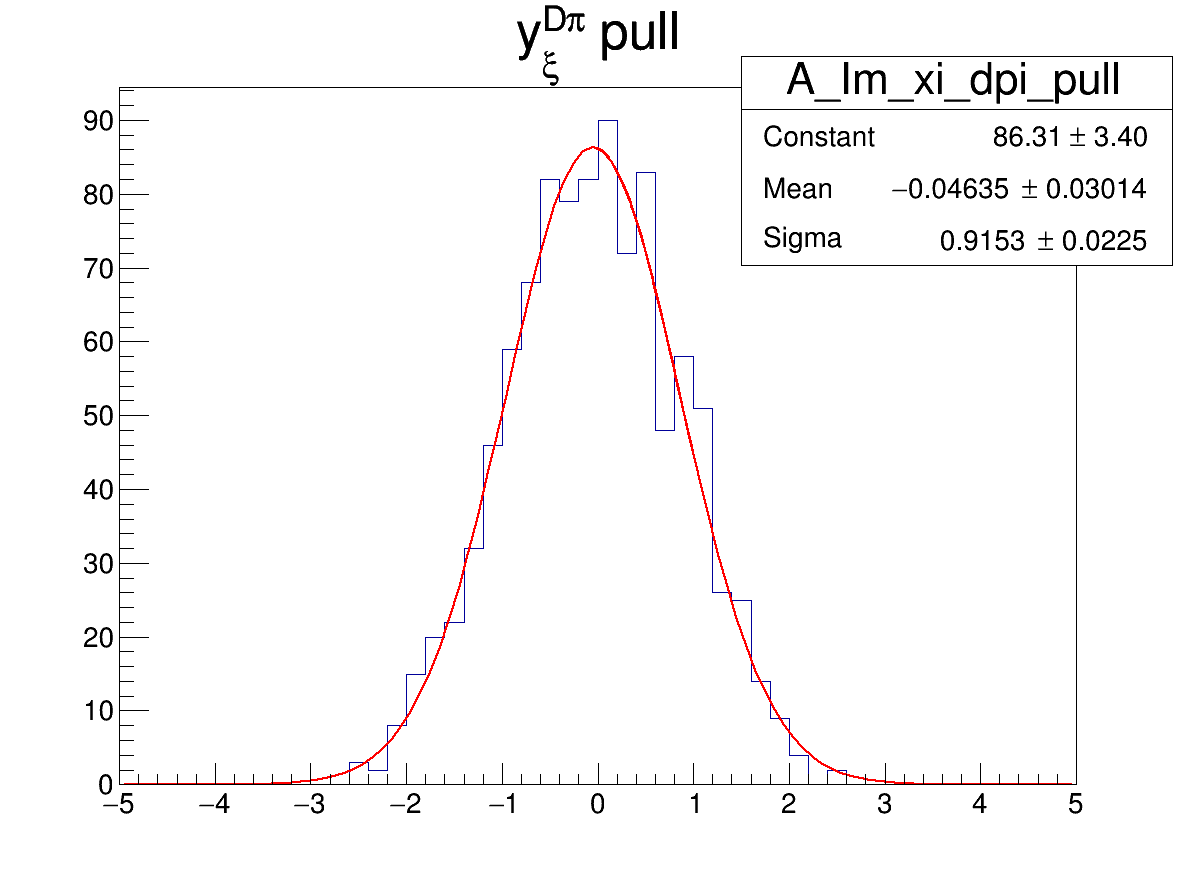
\includegraphics[width = 1.0\textwidth]{A_Im_xi_dpi_8Bins_pull.png}
    \end{subfigure}
    \caption{$B\to D\pi$ CP observable pull distributions}
  \end{figure}
\end{frame}

\begin{frame}{Biases in $B\to D\pi$ CP observables, $8$ bins, $2$x statistics}
  \begin{figure}
    \centering
    \vspace{-0.2cm}
    \begin{subfigure}{0.5\textwidth}
      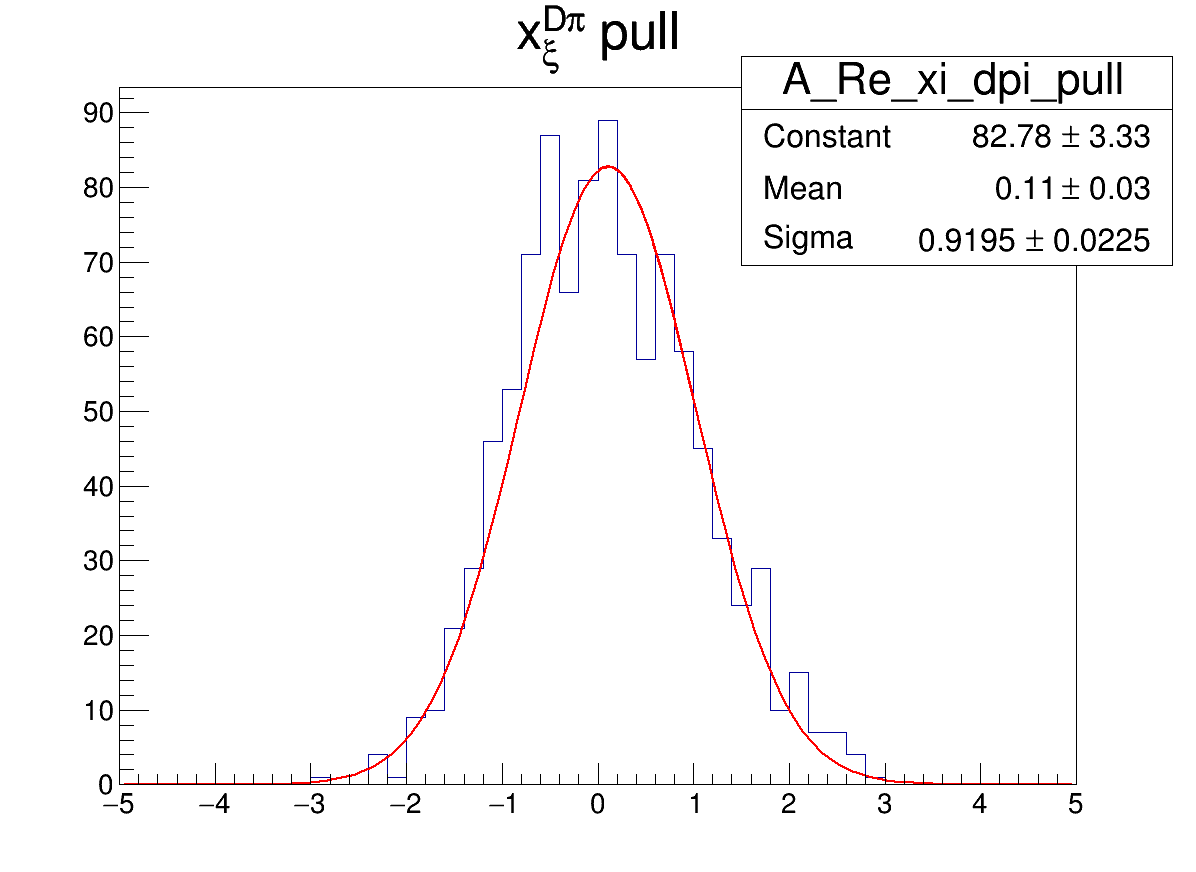
\includegraphics[width = 1.0\textwidth]{A_Re_xi_dpi_8Bins_StatsMultiplier2_pull.png}
    \end{subfigure}%
    \begin{subfigure}{0.5\textwidth}
      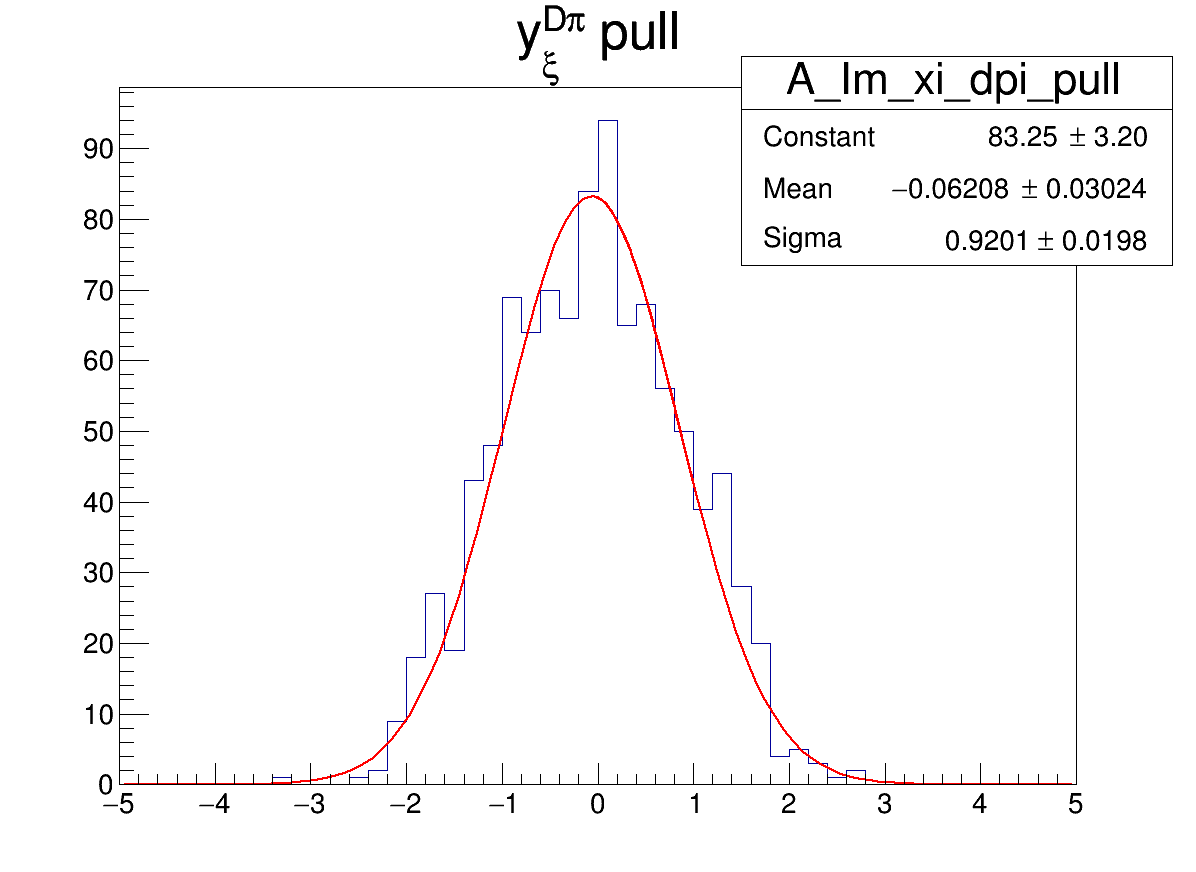
\includegraphics[width = 1.0\textwidth]{A_Im_xi_dpi_8Bins_StatsMultiplier2_pull.png}
    \end{subfigure}
    \caption{$B\to D\pi$ CP observable pull distributions}
  \end{figure}
\end{frame}

\begin{frame}{Biases in $B\to D\pi$ CP observables, $8$ bins, $10$x statistics}
  \begin{figure}
    \centering
    \vspace{-0.2cm}
    \begin{subfigure}{0.5\textwidth}
      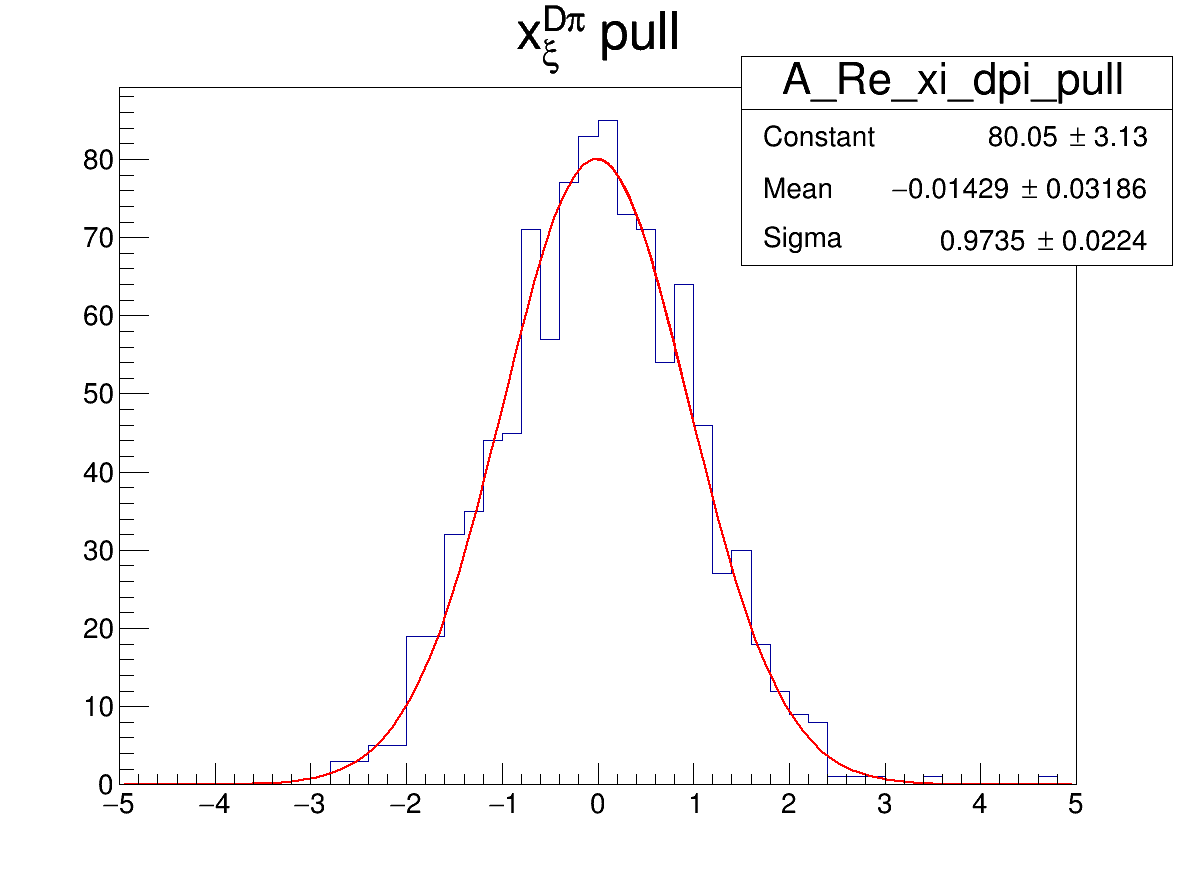
\includegraphics[width = 1.0\textwidth]{A_Re_xi_dpi_8Bins_StatsMultiplier10_pull.png}
    \end{subfigure}%
    \begin{subfigure}{0.5\textwidth}
      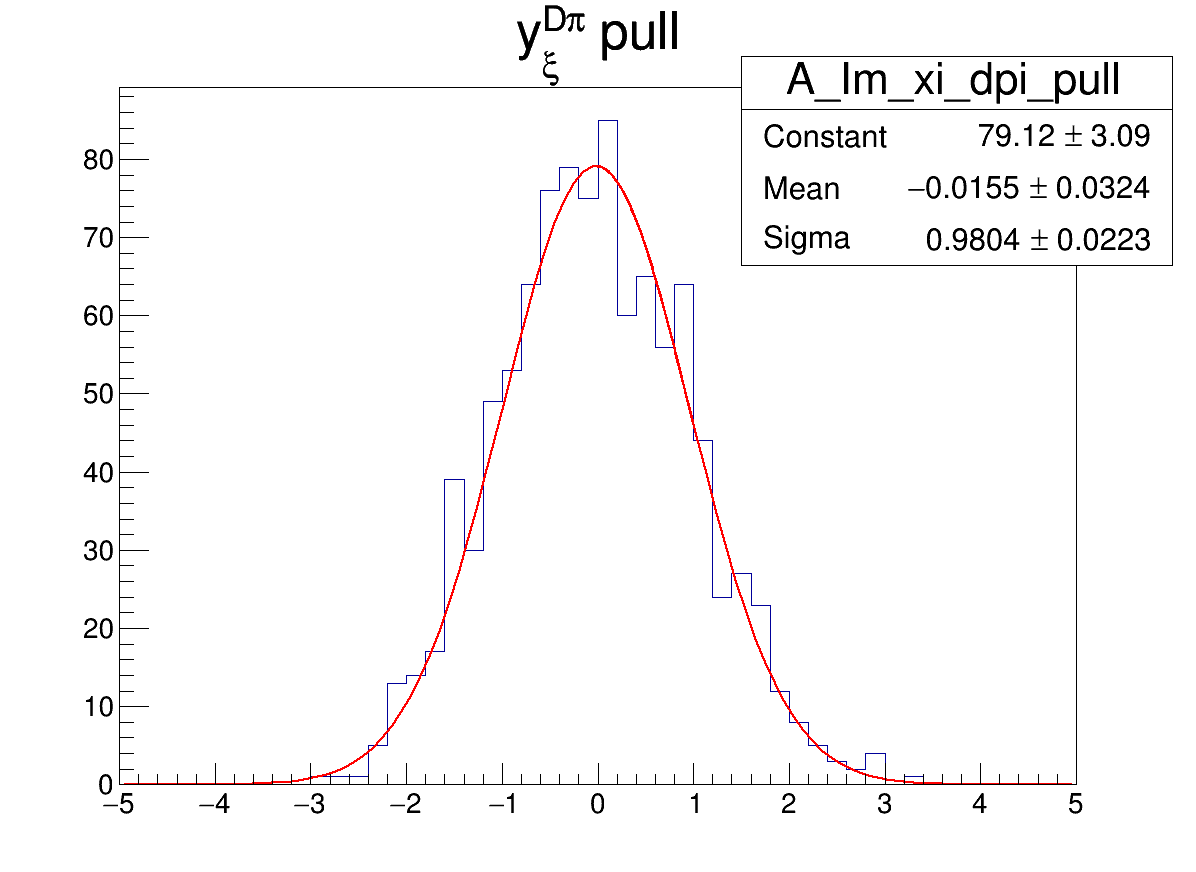
\includegraphics[width = 1.0\textwidth]{A_Im_xi_dpi_8Bins_StatsMultiplier10_pull.png}
    \end{subfigure}
    \caption{$B\to D\pi$ CP observable pull distributions}
  \end{figure}
\end{frame}

\subsection{Systematics from \texorpdfstring{$c_i$, $s_i$}{ci, si}}
\begin{frame}{Systematics from $c_i$, $s_i$}
  \begin{figure}
    \centering
    \vspace{-0.2cm}
    \begin{subfigure}{0.5\textwidth}
      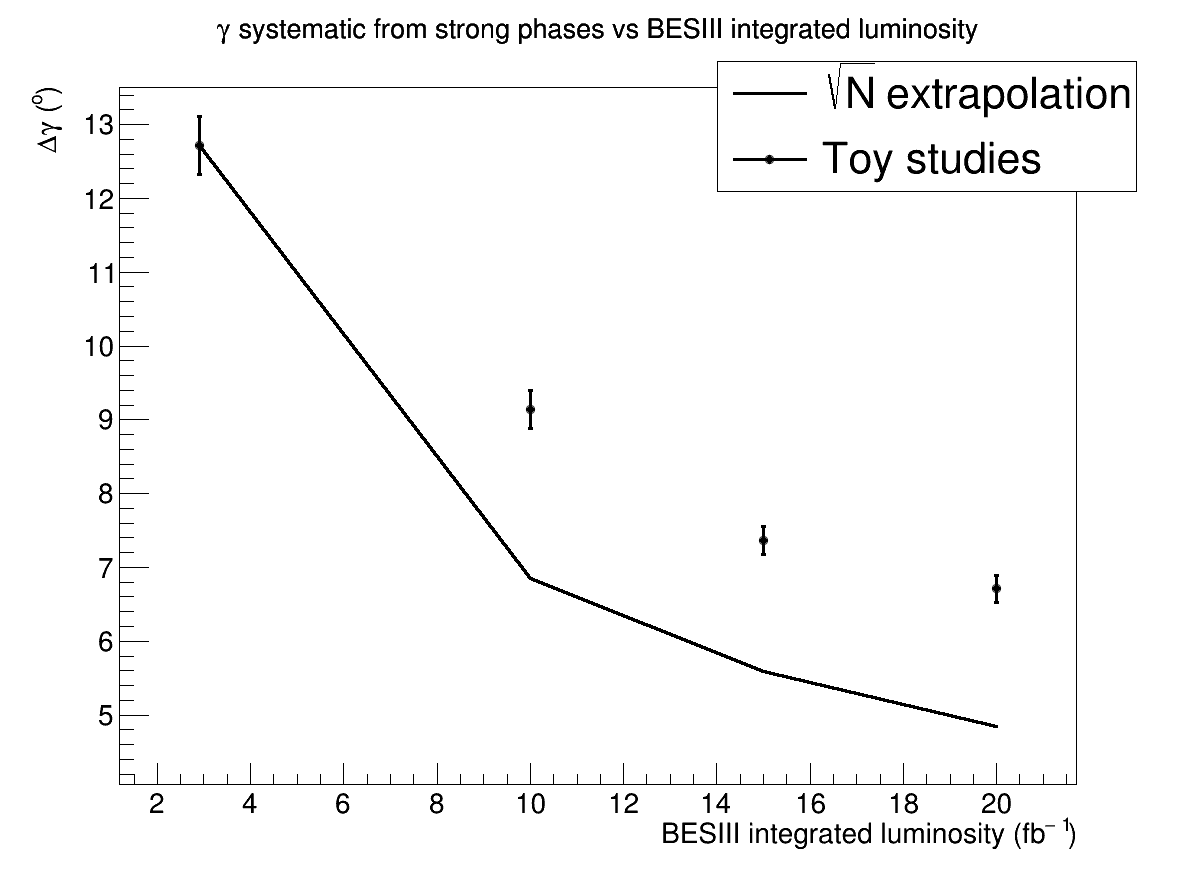
\includegraphics[width = 1.0\textwidth]{cisi_Systematic_4Bins_Run2.png}
      \caption{$4$ bins}
    \end{subfigure}%
    \begin{subfigure}{0.5\textwidth}
      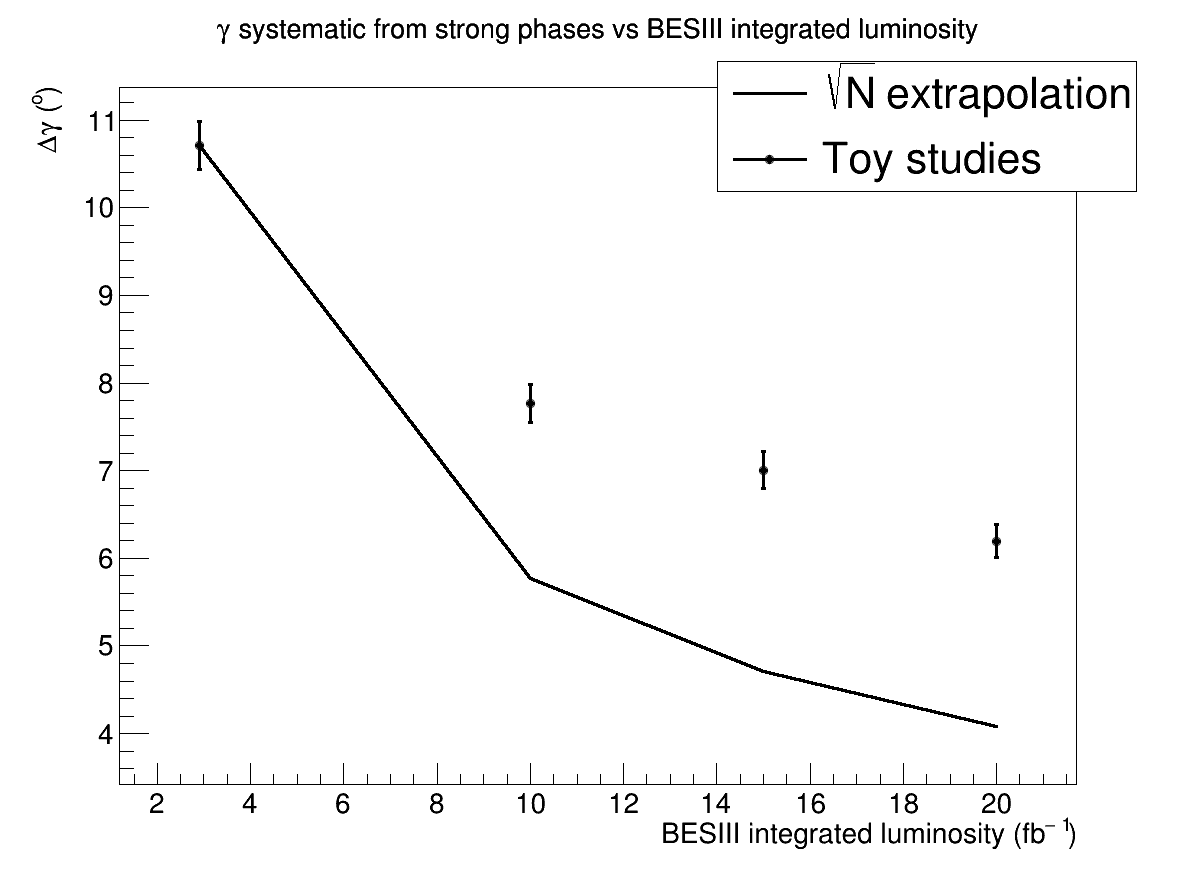
\includegraphics[width = 1.0\textwidth]{cisi_Systematic_8Bins_Run2.png}
      \caption{$8$ bins}
    \end{subfigure}
    \caption{Systematic uncertainty from $c_i$ and $s_i$ with extrapolated BESIII statistics}
  \end{figure}
\end{frame}

\section{Summary and future work}
\begin{frame}{Summary and future work}
  \begin{itemize}
    \item{Summary:}
    \begin{enumerate}
      \setlength\itemsep{1.3em}
      \item{Global mass fit looks promising}
      \item{$D\to K\pi\pi\pi$ and charmless backgrounds under control}
      \item{Toy studies show no suspicious behaviour}
      \item{Expected $c_i$ and $s_i$ systematics are not too large}
    \end{enumerate}
    \item{Next steps:}
    \begin{enumerate}
      \setlength\itemsep{1.3em}
      \item{Study semileptonic backgrounds in RapidSim}
      \item{Recalculate PID efficiencies with PIDCalib}
      \item{Refit MC signal shapes}
      \item{Rerun everything with Run $1$ (finally!)}
    \end{enumerate}
  \end{itemize}
\end{frame}

\end{document}
